\documentclass[12pt]{article}

\usepackage[T1]{fontenc}
\usepackage[utf8]{inputenc}
\usepackage[a4paper,margin=1in]{geometry}
\usepackage{lmodern}
\usepackage{microtype}
\usepackage{xcolor}
\usepackage[hidelinks]{hyperref}
\usepackage{graphicx}
\usepackage{float}
\usepackage{ulem}

\begin{document}

\pagenumbering{gobble}
\begin{titlepage}
    \centering
    
\includegraphics[width=0.15\textwidth]{img/logo.png} \\
    {\large Universidade Federal do Rio Grande do Norte} \\
    {\large Departamento de Informática e Matemática Aplicada} \\
    {\large DIM0124 - Programação Concorrente} \\

    \vfill

    {\LARGE \textbf{Relatório de Desenvolvimento de Aplicação Concorrente}} \\
    \vspace{1cm}
    {\Large \textbf{Algoritmo K-Means}} \\

    \vfill
    
    \raggedright
    {\large Matrícula: 20210081823} \\
    \vspace{0.15cm}
    {\large Nome: Rary Emanuel Gonçalves Coringa} \\
\end{titlepage}

\pagenumbering{arabic}
\tableofcontents
\newpage

\section{Introdução}

\subsection{Descrição do Algoritmo}

O K-Means é um algoritmo de agrupamento não supervisionado que particiona um
conjunto de dados em \(k\) grupos (clusters), de forma que cada ponto pertença
ao cluster cujo centróide é o mais próximo. O algoritmo opera em iterações:
na etapa de \textbf{atribuição}, cada ponto é associado ao centróide mais próximo
segundo a distância euclidiana; na etapa de \textbf{atualização}, cada centróide
é recalculado como a média aritmética de todos os pontos a ele atribuídos. Esse
ciclo se repete até que os centróides estabilizem (deslocamento máximo abaixo de
uma tolerância) ou o número máximo de iterações seja atingido.

A complexidade por iteração é \(O(N \cdot k \cdot d)\), onde \(N\) é o número de
pontos, \(k\) o número de clusters e \(d\) a dimensionalidade dos dados. Por
percorrer todos os pontos a cada iteração, o algoritmo é naturalmente paralelizável
na etapa de atribuição, tornando-o um caso de estudo relevante para comparação
entre estratégias de concorrência.

\subsection{Descrição da Linguagem Erlang}

Erlang é uma linguagem funcional criada pela Ericsson, projetada para sistemas distribuídos e
tolerantes a falhas. Executa sobre a máquina virtual BEAM, que provê concorrência nativa por
meio de processos leves e isolados.

\textbf{Modelo de programação.}
Utiliza passagem de mensagens (modelo de atores). Processos não compartilham memória e se
comunicam exclusivamente via caixas postais, eliminando por construção os problemas de acesso
concorrente a estado compartilhado.

\textbf{Modelo de memória e visibilidade.}
Cada processo possui heap privado. Mensagens são copiadas entre heaps ao ser enviadas, o que
garante isolamento total. Por não haver memória compartilhada mutável, questões de
visibilidade — como barreiras de memória e \texttt{volatile} do Java — não se aplicam.

\textbf{Controle de região crítica.}
Não existem mutexes ou semáforos. O acesso a recursos exclusivos é feito encapsulando-os em
um processo servidor que atende requisições sequencialmente — padrão formalizado pelo
\texttt{gen\_server} OTP.

\textbf{Coleta de lixo.}
O GC opera por processo, de forma independente, sem pausas globais (\textit{stop-the-world}).
Processos de vida curta têm seus heaps simplesmente descartados ao terminar.

\textbf{JIT.}
A partir do OTP 24, a BEAM inclui um compilador JIT (AsmJit) que gera código nativo para
x86-64 e AArch64 no carregamento dos módulos, com ganhos típicos de 20--40\% em relação ao
bytecode interpretado.
\newpage

\section{Configuração dos Experimentos}

\subsection{Configurações do Computador}

Esta seção descreve o ambiente de hardware e software utilizado na execução
dos experimentos. O conhecimento dessas configurações é essencial para a
reprodutibilidade dos resultados e para a correta interpretação das métricas
coletadas.

\subsubsection{Hardware}

\paragraph{CPU:}
O processador utilizado é o \textbf{Intel Core i5-13450HX} (13ª geração), com
arquitetura híbrida composta por 6 P-cores (Performance, com Hyper-Threading)
e 4 E-cores (Efficiency, sem Hyper-Threading), totalizando 10 núcleos físicos
e 16 threads lógicas. A frequência máxima é de 4,6 GHz. As memórias cache são:
L1d 416 KiB, L1i 448 KiB, L2 9,5 MiB e L3 20 MiB.

\paragraph{RAM:}
A memória RAM total é de \textbf{16 GB DDR5} em configuração dual-channel
(2 $\times$ 8 GB).

\paragraph{Disco:}
O armazenamento em disco utilizado é um \textbf{SSD NVMe} com capacidade de
512,1 GB.

\subsubsection{Software}

\paragraph{Sistema Operacional:}
\textbf{Ubuntu 24.04.4 LTS}, kernel \texttt{6.17.0-22-generic}.

\paragraph{Java:}
\textbf{OpenJDK 25.0.1} - Temurin-25.0.1+8 (build 25.0.1+8-LTS).

\paragraph{Erlang:}
\textbf{Erlang/OTP 25}, emulador BEAM versão \texttt{13.2.2.5}, com JIT AsmJit habilitado.
    
\subsection{Configurações de Testes}

\subsubsection{Microbenchmark (JMH)}

Os microbenchmarks foram implementados com \textbf{JMH 1.37} sobre \textbf{JDK 25.0.1},
com modo \texttt{AverageTime}, 1 iteração de aquecimento de 10 s, 3 iterações de
medição de 10 s e 1 fork por benchmark. O dataset é carregado uma única vez antes
das medições e uma semente fixa garante reprodutibilidade dos pontos de teste.

\begin{table}[H]
\centering
\begin{tabular}{llp{7cm}}
\hline
\textbf{ID} & \textbf{Método} & \textbf{Objetivo} \\
\hline
B1 & \texttt{b1\_fullRun}         & Execução completa (\textit{k}=10, maxIter=20, tol=\(10^{-6}\)) — número primário do relatório \\
B2 & \texttt{b2\_perIterationCost} & Execução curta (\textit{k}=10, maxIter=5, tol=0) — isola custo por iteração \\
B3 & \texttt{b3\_closestCentroid}  & Chamada isolada de \texttt{closestCentroid} — ponto quente do laço interno \\
B4 & \texttt{b4\_squaredDistance}  & Chamada isolada de \texttt{squaredDistance} — baseline aritmético \\
\hline
\end{tabular}
\caption{Casos de benchmark JMH definidos em \texttt{KMeansBenchmark}.}
\label{tab:jmh-cases}
\end{table}

A Figura~\ref{fig:jmh-config} apresenta a classe de benchmark com as anotações
de configuração e os quatro métodos medidos.

\begin{figure}[H]
    \centering
    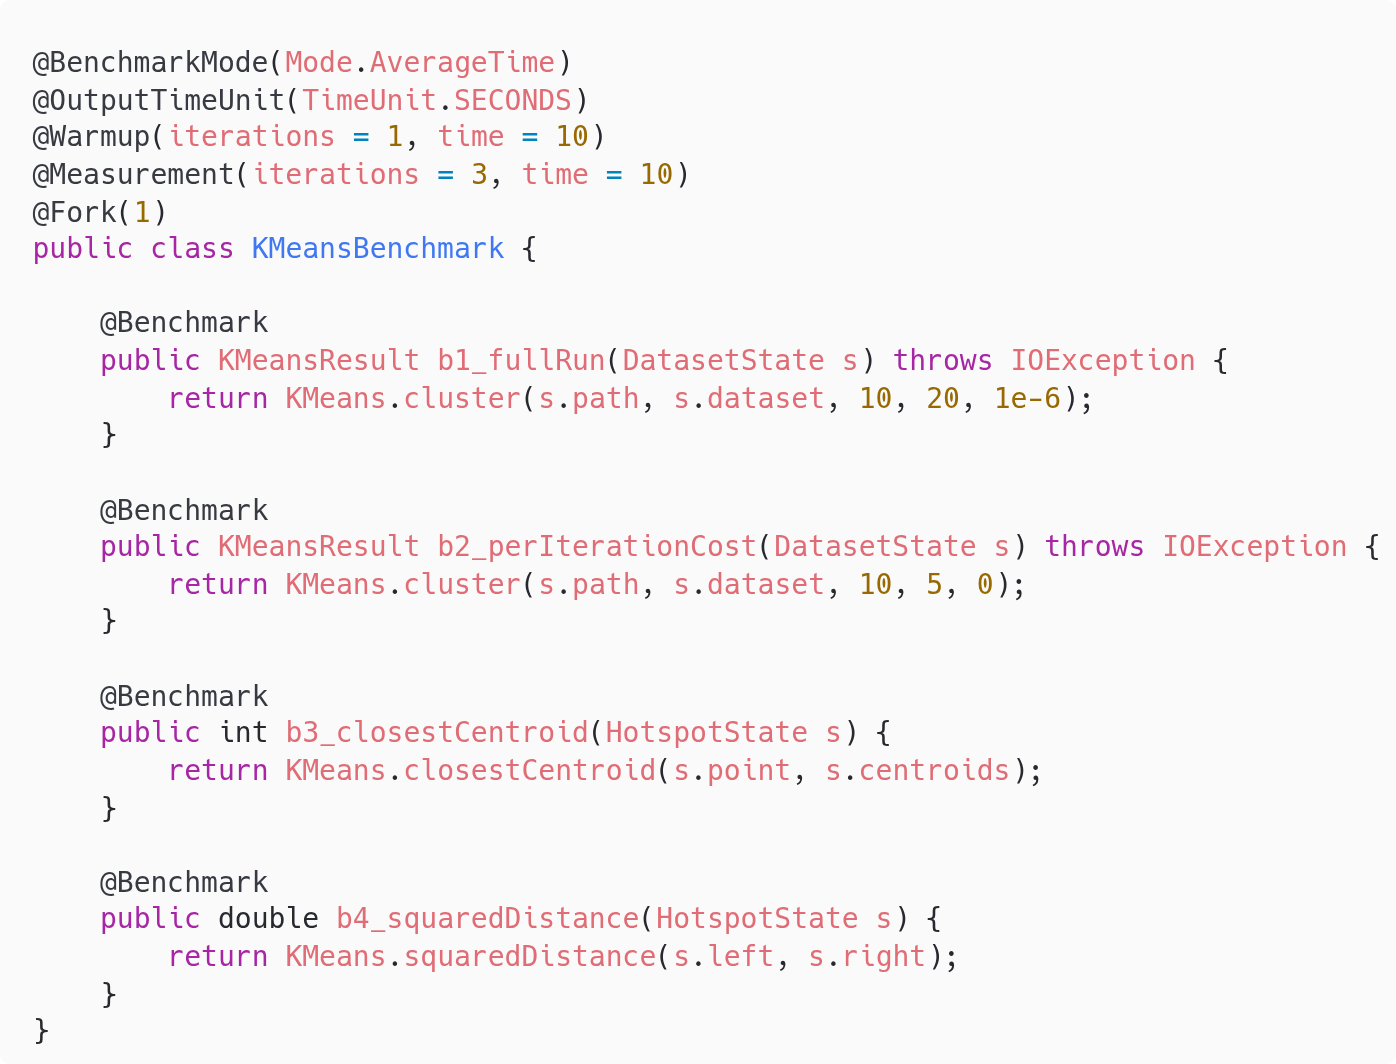
\includegraphics[width=0.85\textwidth]{img/2-configs/jmh-config}
    \caption{Configuração JMH e casos de benchmark em \texttt{KMeansBenchmark}.}
    \label{fig:jmh-config}
\end{figure}

\subsubsection{Macrobenchmark (JMeter)}

Os macrobenchmarks foram implementados com \textbf{Apache JMeter 5.6.3} utilizando
o mecanismo de \textit{Java Sampler} (\texttt{AbstractJavaSamplerClient}). A classe
\texttt{KMeansSampler} executa \texttt{KMeans.cluster()} diretamente na JVM do
JMeter --- sem servidor HTTP intermediário --- permitindo que o coletor de GC
configurado na inicialização do JMeter se aplique integralmente ao algoritmo.

O GC é selecionado pela variável de ambiente \texttt{GC\_ALGO} passada ao script
de inicialização do JMeter. Foram avaliados três coletores:

\begin{itemize}
    \item \texttt{-XX:+UseG1GC} — G1GC (coletor padrão do JDK 25);
    \item \texttt{-XX:+UseZGC} — ZGC (coletor de baixa pausa);
    \item \texttt{-XX:+UseParallelGC} — ParallelGC (coletor paralelo de alta vazão).
\end{itemize}

A matriz de testes combina os três coletores com cinco contagens de threads,
totalizando 15 execuções independentes:

\begin{table}[H]
\centering
\begin{tabular}{ll}
\hline
\textbf{Parâmetro} & \textbf{Valor} \\
\hline
Coletores de GC      & G1GC, ZGC, ParallelGC \\
Threads JMeter       & 1, 2, 4, 8, 16 \\
Duração por execução & 120 s \\
Ramp-up              & 30 s \\
\textit{k}           & 10 \\
maxIter              & 3 \\
tol                  & 0,0 \\
Métrica primária     & Throughput (execuções/min) \\
\hline
\end{tabular}
\caption{Configuração do macrobenchmark JMeter.}
\label{tab:jmeter-config}
\end{table}

\subsubsection{Stress Test (JCStress)}

Os testes de condição de corrida foram implementados com \textbf{JCStress 0.16} e
executados sobre \textbf{JDK 25.0.1}. O JCStress executa múltiplos processos
paralelos variando configurações de compilação e afinidade de CPU, maximizando
a cobertura de possíveis intercalações entre threads.

\begin{table}[H]
\centering
\begin{tabular}{ll}
\hline
\textbf{Parâmetro} & \textbf{Valor} \\
\hline
Ferramenta         & JCStress 0.16 \\
Preset             & \texttt{default} \\
Forks por teste    & 6 (1 normal + 5 stress) \\
Iterações por fork & 5 \\
Tempo por iteração & 1.000 ms \\
CPUs utilizadas    & 16 \\
\hline
\end{tabular}
\caption{Configuração do stress test JCStress.}
\label{tab:jcstress-config}
\end{table}

Foram definidos quatro testes, cada um associado a uma região crítica do algoritmo:

\begin{table}[H]
\centering
\begin{tabular}{llp{6.5cm}}
\hline
\textbf{ID} & \textbf{Classe} & \textbf{Região crítica} \\
\hline
JCS1 & \texttt{JCS1\_ClosestCentroidTest}       & Leitura concorrente do snapshot de centróides \\
JCS2 & \texttt{JCS2\_SquaredDistanceTest}        & Leitura concorrente de \texttt{double[]} compartilhado \\
JCS3 & \texttt{JCS3\_LocalCountAccumulationTest} & \texttt{counts[0]++} em array compartilhado (abordagem ingênua) \\
JCS4 & \texttt{JCS4\_LocalSumAccumulationTest}   & \texttt{sums[0] += 1.0} em array compartilhado (abordagem ingênua) \\
\hline
\end{tabular}
\caption{Testes JCStress e regiões críticas associadas.}
\label{tab:jcstress-tests}
\end{table}

\subsubsection{Profile (JFR)}

O profile foi capturado com \textbf{JFR (Java Flight Recorder)}, ferramenta embutida
no JDK 25 --- sem necessidade de instalação adicional. A gravação foi iniciada via
flag de JVM na execução do algoritmo e analisada exclusivamente com a ferramenta
de linha de comando \texttt{jfr} do JDK, sem uso do JMC (\textit{Java Mission Control}).

A configuração \texttt{settings=profile} habilita amostragem de CPU em alta resolução
(intervalo de 10 ms), adequada para identificar hot methods. A flag
\texttt{dumponexit=true} garante que o arquivo \texttt{.jfr} seja gravado ao final
da execução mesmo sem intervenção manual.

\begin{table}[H]
\centering
\begin{tabular}{ll}
\hline
\textbf{Parâmetro} & \textbf{Valor} \\
\hline
Ferramenta         & JFR (JDK 25 built-in) \\
Configuração       & \texttt{settings=profile} \\
Captura            & \texttt{dumponexit=true} \\
Análise            & \texttt{jfr print} (CLI) \\
GC                 & G1GC \\
\textit{k}         & 10 \\
maxIter            & 3 \\
Dataset            & $\approx$1 GB \\
\hline
\end{tabular}
\caption{Configuração do profile JFR.}
\label{tab:jfr-config}
\end{table}

Os eventos analisados cobrem quatro áreas:

\begin{itemize}
    \item amostras de CPU por método (identificação dos hot methods);
    \item pausas e uso de heap do coletor de GC;
    \item carga de CPU por thread e número de threads ativas;
    \item eventos de leitura de arquivo (bytes lidos, duração).
\end{itemize}

\subsubsection{Microbenchmark em Erlang}

Os microbenchmarks Erlang utilizam \texttt{timer:tc/1}, função nativa do OTP que
mede o tempo de execução de uma fun com resolução de microssegundos. São executadas
1 iteração de aquecimento e 3 de medição, com o dataset carregado uma única vez em
memória antes de qualquer medição para eliminar o custo de I/O dos resultados.
São medidos três casos equivalentes ao JMH: execução completa do algoritmo (B1),
\texttt{closest\_centroid} isolado (B3) e \texttt{squared\_distance} isolado (B4).

\subsubsection{Profile em Erlang}

O profile Erlang coleta métricas de tempo e GC via funções nativas do OTP, sem
necessidade de ferramentas externas. São capturados: tempo de CPU, tempo de parede,
número de coletas GC e utilização média dos schedulers BEAM. O profile cobre uma
execução completa do algoritmo com $k=10$ e \texttt{maxIter}=10.
\newpage

\section{Implementação Serial}

\subsection{Implementação em Java}

\subsubsection{Descrição}

A implementação serial em Java é composta por quatro classes principais, cada uma
com responsabilidade bem delimitada:

\begin{itemize}
    \item \texttt{CsvDataset} — lê o cabeçalho do arquivo CSV e expõe os dados
          linha a linha via \texttt{forEachPoint}, sem carregar o dataset inteiro
          em memória;
    \item \texttt{KMeans} — contém o algoritmo K-Means: inicialização dos
          centróides, laço de atribuição e recomputo, verificação de convergência
          e avaliação final;
    \item \texttt{KMeansResult} — registro imutável que armazena os centróides
          finais, tamanhos de cluster, número de iterações e soma dos erros
          quadráticos;
    \item \texttt{Main} — ponto de entrada; configura \(k = 10\),
          \texttt{maxIter} = 10 e \texttt{tolerance} = \(10^{-6}\) e imprime o
          resumo dos clusters ao final.
\end{itemize}

\begin{figure}[H]
  \centering
  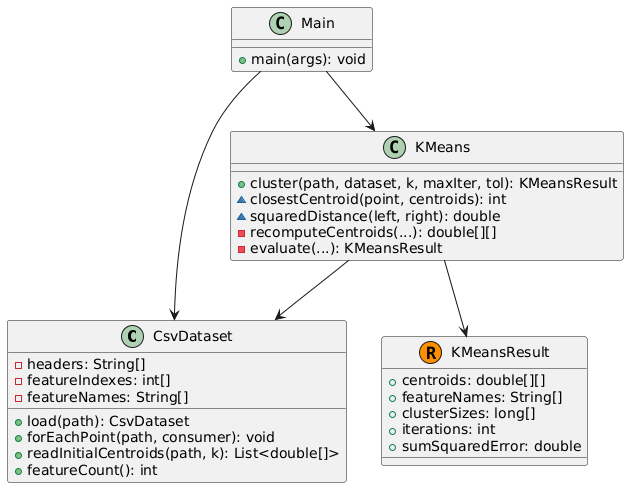
\includegraphics[width=0.6\textwidth]{img/3-serial/class-diagram}
  \caption{Diagrama de classes da implementação serial em Java.}
  \label{fig:class-diagram-serial-java}
\end{figure}

O dataset é processado em modo \textit{streaming}: a cada iteração do algoritmo,
\texttt{forEachPoint} abre o arquivo, lê e descarta o cabeçalho, e entrega cada
linha decodificada ao consumidor sem acumular pontos na memória heap. A
Figura~\ref{fig:snippet-foreach} mostra essa interface.

\begin{figure}[H]
    \centering
    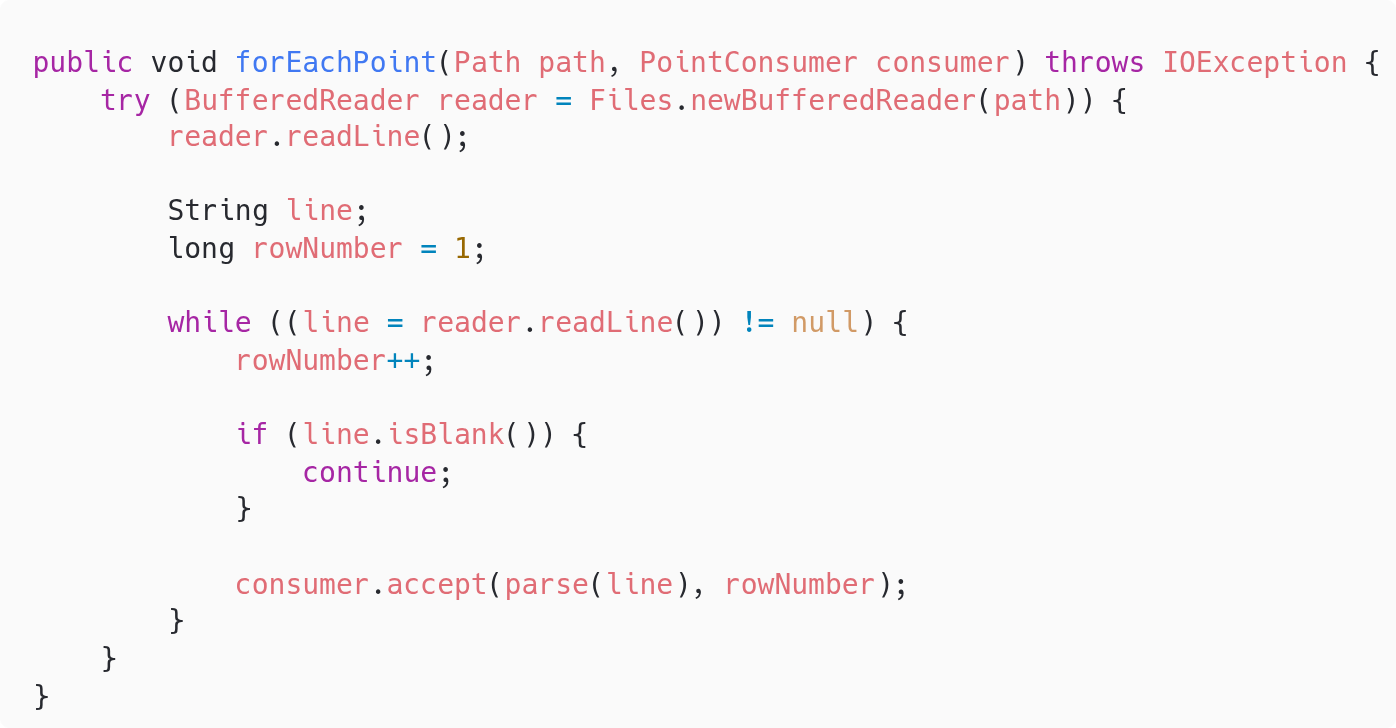
\includegraphics[width=0.85\textwidth]{img/3-serial/snippet-1}
    \caption{Leitura linha a linha do dataset (\texttt{CsvDataset.forEachPoint}).}
    \label{fig:snippet-foreach}
\end{figure}

O laço principal do algoritmo, mostrado na Figura~\ref{fig:snippet-cluster-loop},
percorre todos os pontos a cada iteração para acumular somas parciais e contagens
por cluster, e em seguida recomputa os centróides dividindo as somas pelas
contagens.

\begin{figure}[H]
    \centering
    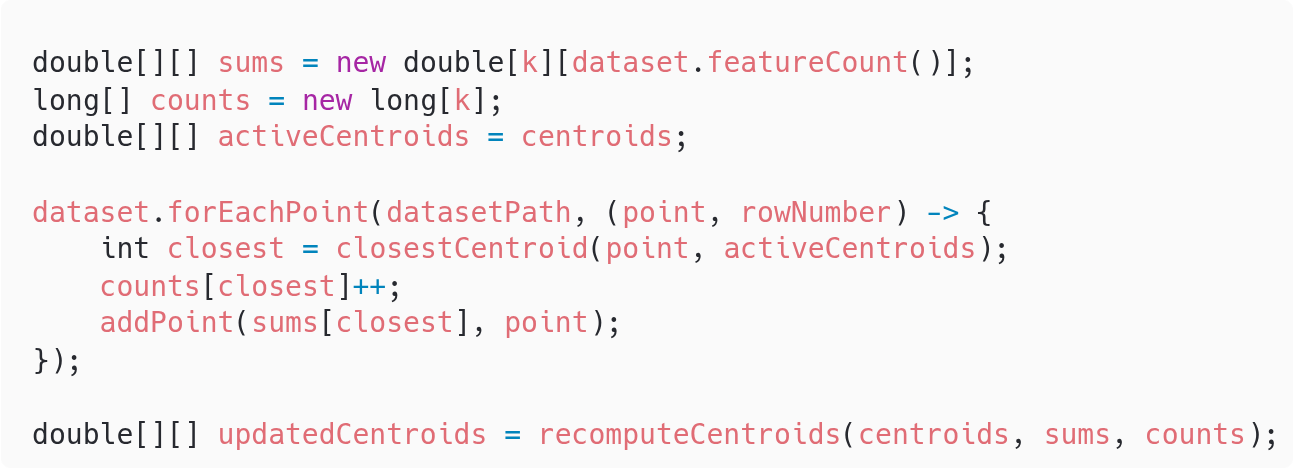
\includegraphics[width=0.85\textwidth]{img/3-serial/snippet-2}
    \caption{Laço de atribuição e recomputo de centróides (\texttt{KMeans.cluster}).}
    \label{fig:snippet-cluster-loop}
\end{figure}

A função \texttt{closestCentroid} (Figura~\ref{fig:snippet-closest}) varre os \(k\)
centróides para cada ponto e retorna o índice do mais próximo usando distância
euclidiana ao quadrado, evitando a raiz quadrada desnecessária. Essa função é
o principal ponto quente da CPU, executada \(N \times k\) vezes por iteração.

\begin{figure}[H]
    \centering
    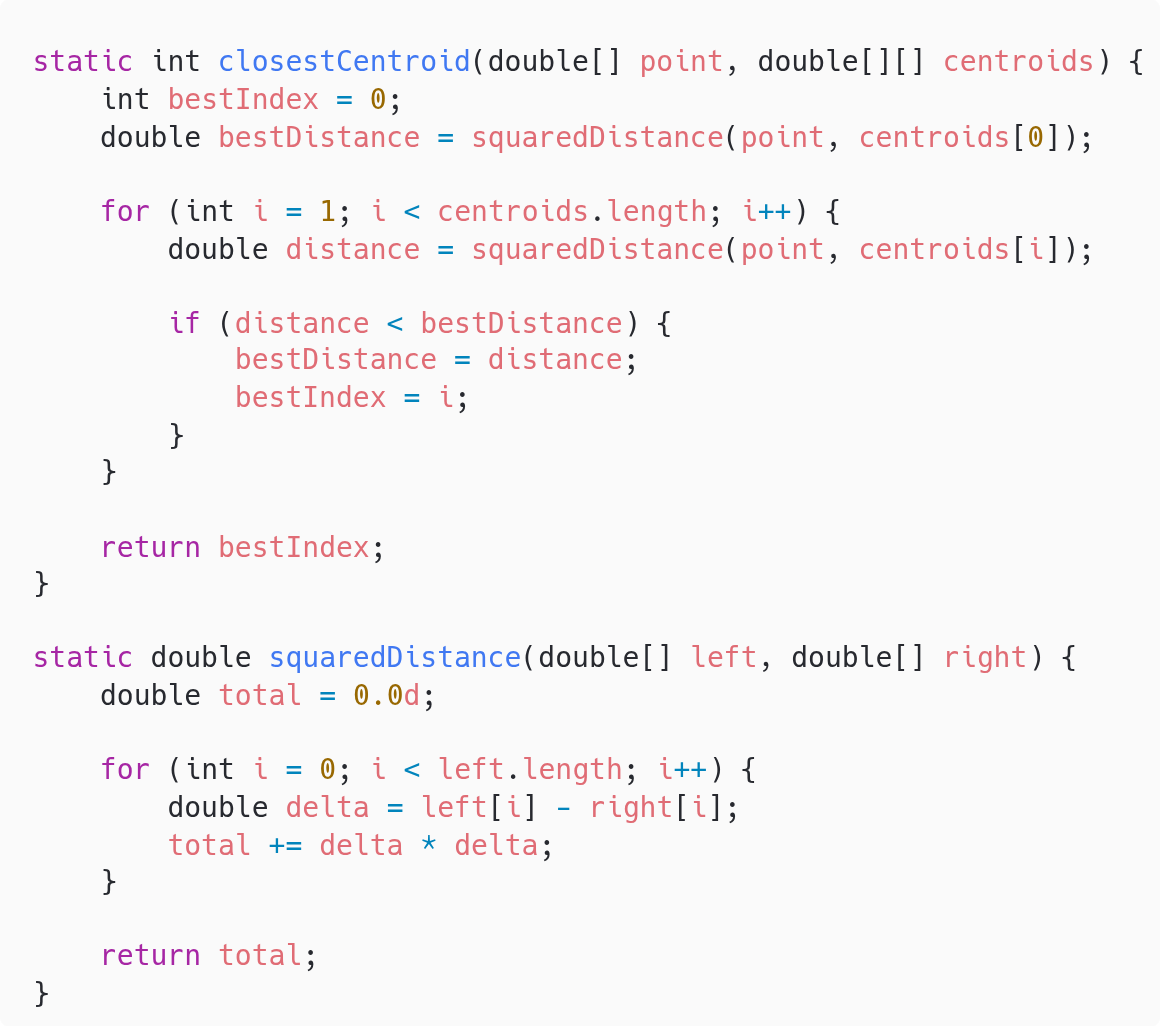
\includegraphics[width=0.85\textwidth]{img/3-serial/snippet-3}
    \caption{Busca do centróide mais próximo e distância euclidiana ao quadrado.}
    \label{fig:snippet-closest}
\end{figure}

\subsubsection{Resultados}

\paragraph{Avaliação com Microbenchmark}

Os microbenchmarks foram executados com JMH 1.37 sobre JDK 25.0.1 (OpenJDK 64-Bit
Server VM), com 1 fork, 1 iteração de aquecimento de 10 s e 3 iterações de medição
de 10 s cada. O dataset utilizado possui aproximadamente 1 GB de dados de pedidos
sintéticos.

\begin{table}[h]
\centering
\begin{tabular}{llrrr}
\hline
\textbf{ID} & \textbf{Benchmark} & \textbf{Média} & \textbf{Erro ($\pm$)} & \textbf{Unidade} \\
\hline
B1 & Execução completa (\textit{k}=10, maxIter=20) & 212{,}57 & 34{,}48 & s/op \\
B2 & Custo por iteração (\textit{k}=10, maxIter=5)  &  60{,}05 &  2{,}46 & s/op \\
B3 & \texttt{closestCentroid} (\textit{k}=10, 38 dims) &  96{,}82 &  5{,}59 & ns/op \\
B4 & \texttt{squaredDistance} (38 dims)               &   9{,}31 &  1{,}41 & ns/op \\
\hline
\end{tabular}
\caption{Resultados JMH para a implementação serial em Java.}
\label{tab:jmh-serial-java}
\end{table}

B2 mostra que cada iteração leva cerca de 12 s, dominado pela releitura do CSV a cada
ciclo. B3 e B4 mostram que o cálculo aritmético é rápido (96 ns e 9 ns por chamada).
O gargalo não está na CPU, mas na leitura e no parsing do arquivo.

% Mostrar tabela de resultados comparando Java com a linguagem escolhida

\paragraph{Avaliação com Macrobenchmark}

Os macrobenchmarks foram executados com JMeter 5.6.3 sobre JDK 25.0.1, com
\(k = 10\), \texttt{maxIter} = 3 e \texttt{tol} = 0,0. Cada configuração
(GC $\times$ threads) rodou por 120 s com ramp-up de 30 s. A
Tabela~\ref{tab:jmeter-serial-java} apresenta a throughput obtida em cada combinação.

\begin{table}[H]
\centering
\begin{tabular}{rrrrr}
\hline
\textbf{Threads} & \textbf{G1GC} & \textbf{ZGC} & \textbf{ParallelGC} & \textbf{Unidade} \\
\hline
1  & 1,56 & 1,50 & 1,52 & execuções/min \\
2  & 2,25 & 2,01 & 2,26 & execuções/min \\
4  & 2,70 & 2,54 & 2,79 & execuções/min \\
8  & 3,44 & 3,23 & 3,51 & execuções/min \\
16 & 4,66 & 4,40 & 4,85 & execuções/min \\
\hline
\end{tabular}
\caption{Throughput por número de threads e coletor de GC --- implementação serial em Java.}
\label{tab:jmeter-serial-java}
\end{table}

O throughput cresce com o número de threads JMeter, mas com retornos decrescentes:
de 1 para 16 threads, o ganho é de $\approx$3$\times$. A latência piora com mais
threads, pois todas as instâncias leem o mesmo arquivo de $\approx$1 GB ao mesmo
tempo, saturando a I/O do disco.

\paragraph{Avaliação de Profile}

O profile foi capturado com JFR (\texttt{settings=profile}) sobre uma execução completa
do algoritmo serial (\(k=10\), \texttt{maxIter=3}, G1GC, dataset $\approx$1 GB).
A gravação durou 118 s e foi analisada com a ferramenta \texttt{jfr} do JDK 25.

\textbf{Hot Methods.}
A Tabela~\ref{tab:jfr-hot-methods} apresenta os métodos com maior frequência de
amostragem de CPU (\texttt{jdk.ExecutionSample}, 11.054 amostras no total).

\begin{table}[H]
\centering
\begin{tabular}{lrrl}
\hline
\textbf{Método} & \textbf{Amostras} & \textbf{CPU (\%)} & \textbf{Categoria} \\
\hline
\texttt{FloatingDecimal.readJavaFormatString} & 2784 & 25,2 & Parsing CSV \\
\texttt{String.split}                         & 1873 & 16,9 & Parsing CSV \\
\texttt{FloatingDecimal.copyDigits}           & 1817 & 16,4 & Parsing CSV \\
\texttt{FloatingDecimal.parseDouble}          & 1782 & 16,1 & Parsing CSV \\
\texttt{FloatingDecimal.doubleValue}          &  831 &  7,5 & Parsing CSV \\
\texttt{KMeans.squaredDistance}               &  638 &  5,8 & Algoritmo   \\
\texttt{BufferedReader.readLine}              &  609 &  5,5 & I/O         \\
\texttt{KMeans.closestCentroid}               &  205 &  1,9 & Algoritmo   \\
\texttt{KMeans.addPoint}                      &   33 &  0,3 & Algoritmo   \\
\hline
\end{tabular}
\caption{Hot methods na implementação serial em Java (JFR, 11.054 amostras).}
\label{tab:jfr-hot-methods}
\end{table}

O parsing CSV (\texttt{String.split} + \texttt{Double.parseDouble} e suas
dependências internas) consome $\approx$82\% do tempo de CPU, revelando que o
gargalo real não é a leitura de disco em si, mas a conversão de texto para
\texttt{double} linha a linha. O código aritmético do K-Means
(\texttt{squaredDistance} + \texttt{closestCentroid} + \texttt{addPoint})
representa apenas $\approx$8\% — coerente com os resultados JMH de B3 (96 ns/op)
e B4 (9 ns/op).

\textbf{GC.}
Foram realizadas 1.099 coletas Young GC em 118 s (9,3/s), com pausa total de
805 ms — apenas 0,68\% do tempo de execução. O heap oscila entre
$\approx$150 MB e $\approx$5 MB após cada coleta, reflexo da alta taxa de
criação e descarte de objetos \texttt{String} durante o parsing. O GC não é
um gargalo.

\textbf{Threads.}
Uma única thread de trabalho executa todo o algoritmo; as demais 7 threads
são internas da JVM (GC, compilador JIT, etc.). Não há contenção nem
paralelismo.

\textbf{Síntese.}
O principal gargalo é o parsing CSV (\texttt{String.split} + \texttt{Double.parseDouble}),
que consome $\approx$82\% do CPU. O cálculo aritmético do K-Means representa apenas $\approx$8\%.

\iffalse % ============================================================
% ERLANG — seção desativada, manter para uso futuro
\subsection{\sout{Implementação em Erlang}}

\subsubsection{\sout{Descrição}}

% Descrever como o algoritmo foi implementado na outra linguagem

\subsubsection{\sout{Resultados}}

\paragraph{\sout{Avaliação com Microbenchmark}}

\paragraph{\sout{Avaliação com Macrobenchmark}}

\paragraph{\sout{Avaliação de Profile}}
\fi % ============================================================

\subsection{Discussão}

\textbf{Trechos caros e candidatos à concorrência.}
O JFR mostra que $\approx$82\% do CPU é gasto com parsing CSV
(\texttt{String.split} + \texttt{Double.parseDouble}). O laço de atribuição,
que chama \texttt{closestCentroid} $N \times k$ vezes por iteração, é
independente entre pontos e é o principal candidato à paralelização. A
releitura do arquivo a cada iteração (\texttt{forEachPoint}) é outro gargalo
que poderia ser eliminado carregando o dataset em memória.

\textbf{Comparação de coletores de GC.}
A Tabela~\ref{tab:jmeter-serial-gc} compara o throughput por coletor em três
níveis de carga.

\begin{table}[H]
\centering
\begin{tabular}{lrrrr}
\hline
\textbf{GC} & \textbf{1 thread} & \textbf{4 threads} & \textbf{16 threads} & \textbf{Unidade} \\
\hline
G1GC       & 1{,}56 & 2{,}70 & 4{,}66 & execuções/min \\
ZGC        & 1{,}50 & 2{,}54 & 4{,}40 & execuções/min \\
ParallelGC & 1{,}52 & 2{,}79 & 4{,}85 & execuções/min \\
\hline
\end{tabular}
\caption{Throughput por coletor de GC --- implementação serial.}
\label{tab:jmeter-serial-gc}
\end{table}

O ParallelGC tem o maior throughput em todos os níveis, seguido pelo G1GC. O ZGC
fica levemente atrás: mesmo com baixa pressão de heap, as barreiras de escrita do
seu algoritmo adicionam custo. No geral, o impacto do GC é pequeno --- as pausas
somam menos de 1\% do tempo total.

\newpage

\section{Implementação Concorrente}

\subsection{Implementação em Java}

\subsubsection{Descrição}

A estrutura geral do algoritmo é mantida em relação à versão serial: inicializar
centróides, iterar entre atribuição e recomputo, verificar convergência. O que muda
é \textit{como} os pontos são processados dentro de cada iteração.

Na versão serial, a thread principal lê cada ponto diretamente do arquivo, chama
\texttt{closestCentroid} e acumula os resultados em arrays compartilhados. Na versão
concorrente, a leitura ainda é feita sequencialmente, mas os pontos são agrupados em
lotes (\texttt{BATCH\_SIZE = 5.000}) e cada lote é submetido ao pool de workers como
uma tarefa independente. Os workers acumulam em arrays \emph{locais} e retornam um
\texttt{PartialResult}; a thread coordenadora reduz todos os parciais após coletar
os \texttt{Future}s.

Esse padrão --- \emph{dispatch em lotes, acumulação local, redução sequencial} ---
elimina a necessidade de sincronização nas regiões críticas CR1--CR4 sem uso de
\texttt{synchronized} ou variáveis atômicas. A chamada \texttt{Future.get()} garante
a relação happens-before entre a escrita dos workers e a leitura da coordenadora.

Uma cópia imutável dos centróides (\texttt{snapshot}) é tirada antes do dispatch de
cada iteração, garantindo que todos os workers vejam o mesmo estado de centróides
durante a iteração em andamento.

Foram implementadas três variantes concorrentes:

\begin{itemize}
    \item \textbf{v2-platform} --- pool fixo de $N$ platform threads para os workers
          e a thread \texttt{main} como coordenadora.
    \item \textbf{v2-virtual} --- pool fixo de $N$ virtual threads para os workers,
          mesma estrutura de v2-platform.
    \item \textbf{v2-hybrid} --- pool fixo de $N$ platform threads como workers
          CPU-bound e uma virtual thread como coordenadora
          (\texttt{newVirtualThreadPerTaskExecutor}). A virtual thread desmonta
          automaticamente durante \texttt{readLine} (I/O de disco) e durante cada
          \texttt{Future.get()} (park), liberando o carrier sem bloquear o
          \texttt{ForkJoinPool}.
\end{itemize}

As classes \texttt{CsvDataset}, \texttt{KMeansResult} e \texttt{Main} não foram
alteradas. As adições ficaram concentradas em \texttt{KMeans.java}:
dois records privados (\texttt{PartialResult}, \texttt{EvaluatePartial}) e três
métodos novos (\texttt{runClustering}, \texttt{processAssignBatch},
\texttt{processEvaluateBatch}). O método \texttt{evaluate} foi refatorado para
também usar o pool de workers. A classe \texttt{KMeansSampler} foi adicionada como
adaptador JMeter para os macrobenchmarks.

O diagrama de classes da Figura~\ref{fig:class-diagram-concurrent-java} mostra as
classes do projeto com as adições da versão concorrente em destaque.

\begin{figure}[H]
  \centering
  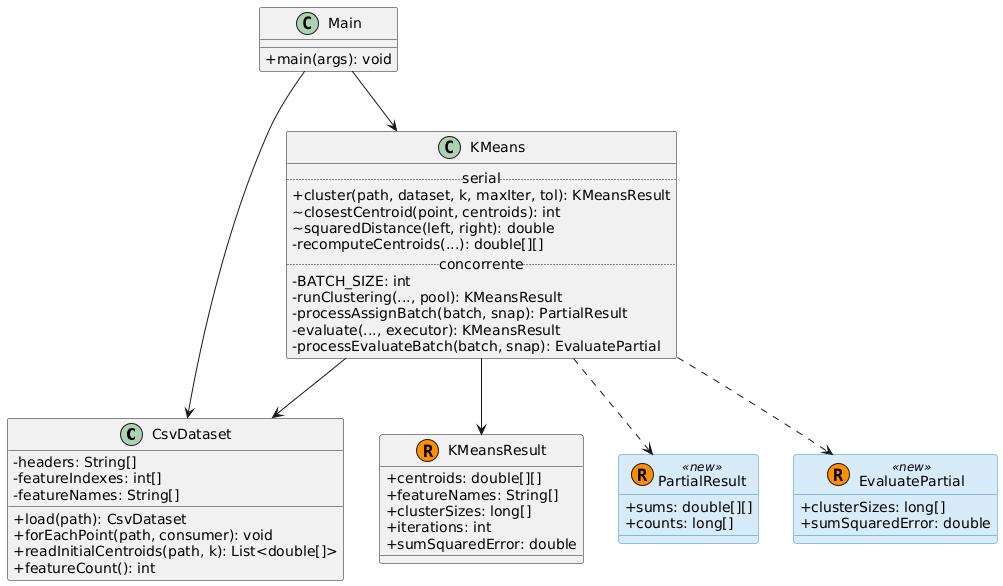
\includegraphics[width=0.85\textwidth]{img/4-concurrent/class-diagram}
  \caption{Diagrama de classes da implementação concorrente em Java. Elementos
           destacados são novos em relação à versão serial.}
  \label{fig:class-diagram-concurrent-java}
\end{figure}

A Figura~\ref{fig:snippet-concurrent-cluster} mostra a criação dos dois executores
e a submissão do método coordenador à virtual thread.

\begin{figure}[H]
  \centering
  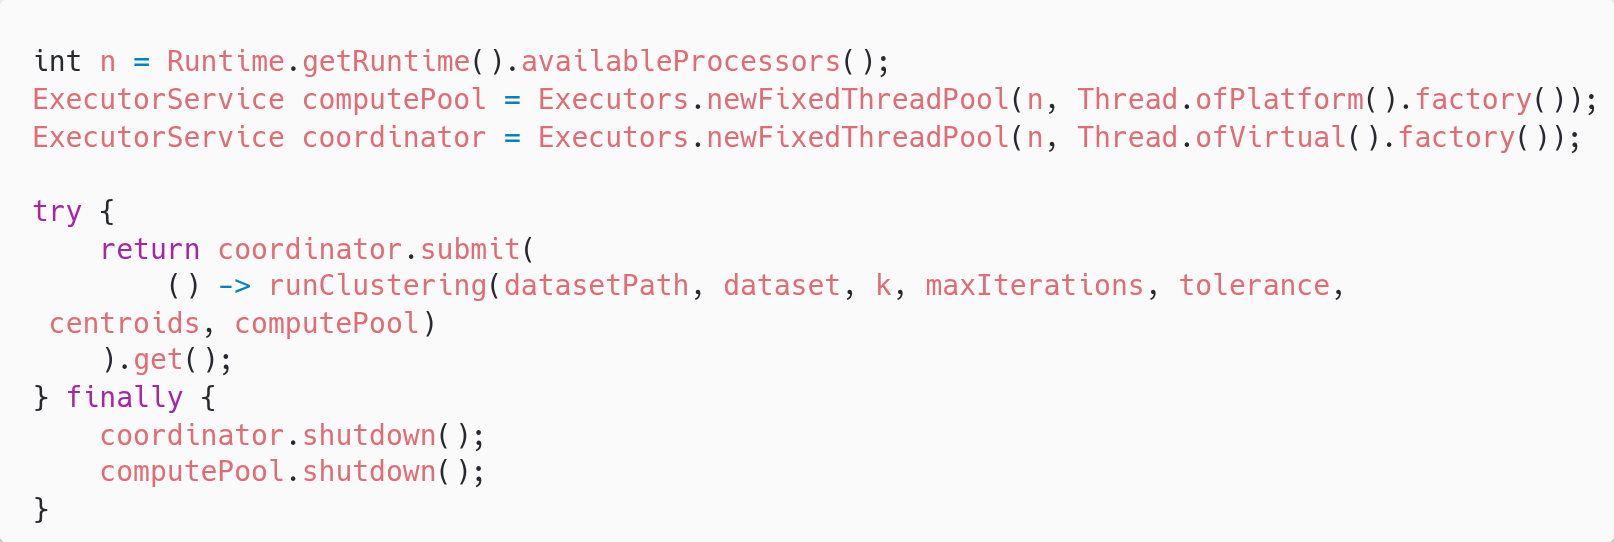
\includegraphics[width=0.85\textwidth]{img/4-concurrent/snippet-1}
  \caption{Criação dos executores e submissão do coordenador (\texttt{KMeans.cluster}).}
  \label{fig:snippet-concurrent-cluster}
\end{figure}

A Figura~\ref{fig:snippet-concurrent-dispatch} mostra o laço de dispatch de lotes
dentro de \texttt{runClustering}: a leitura sequencial acumula pontos até atingir
\texttt{BATCH\_SIZE}, quando cada lote é submetido ao pool e o buffer é esvaziado.

\begin{figure}[H]
  \centering
  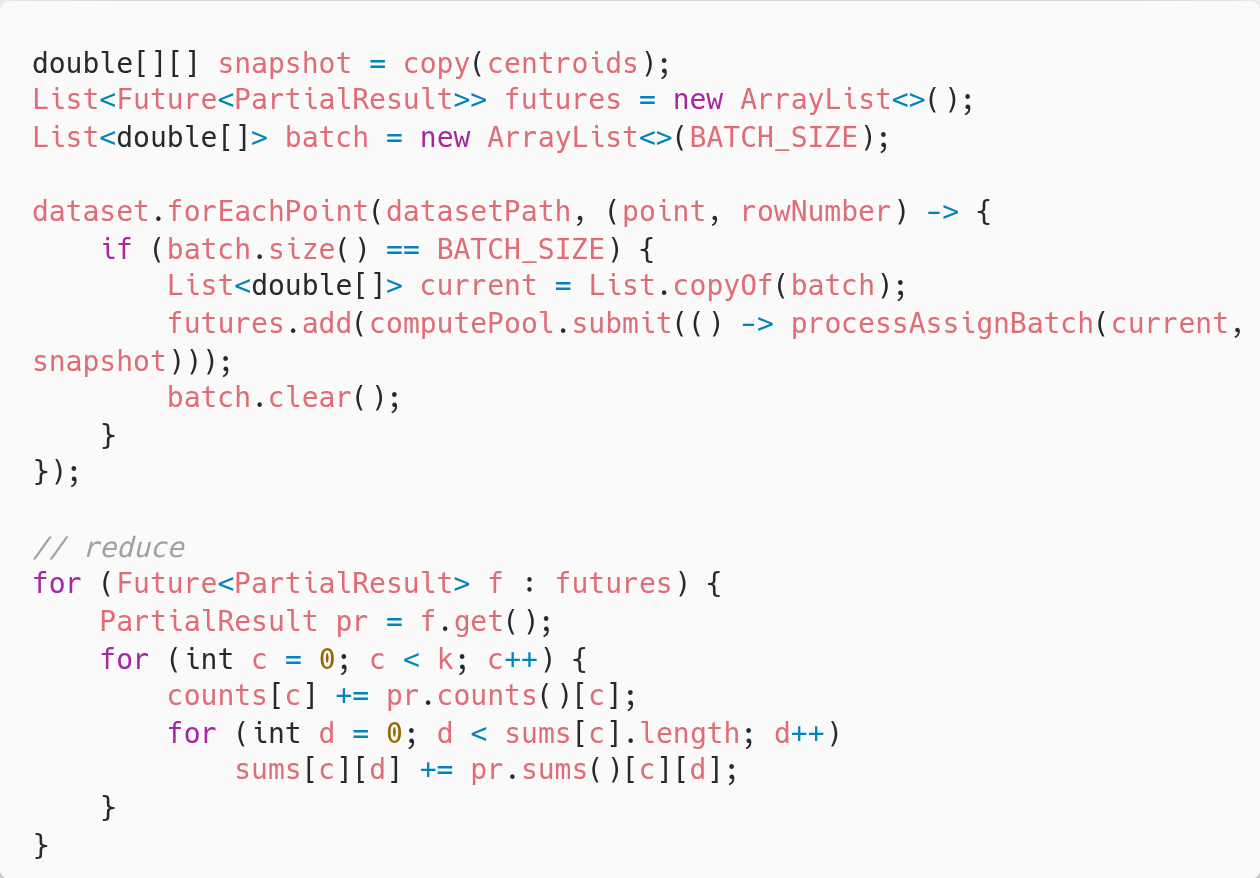
\includegraphics[width=0.85\textwidth]{img/4-concurrent/snippet-2}
  \caption{Dispatch de lotes e coleta de futures (\texttt{KMeans.runClustering}).}
  \label{fig:snippet-concurrent-dispatch}
\end{figure}

A Figura~\ref{fig:snippet-concurrent-batch} mostra \texttt{processAssignBatch}, o
método executado por cada worker: usa arrays locais (\texttt{localSums},
\texttt{localCounts}) sem compartilhamento, retornando um \texttt{PartialResult}
imutável.

\begin{figure}[H]
  \centering
  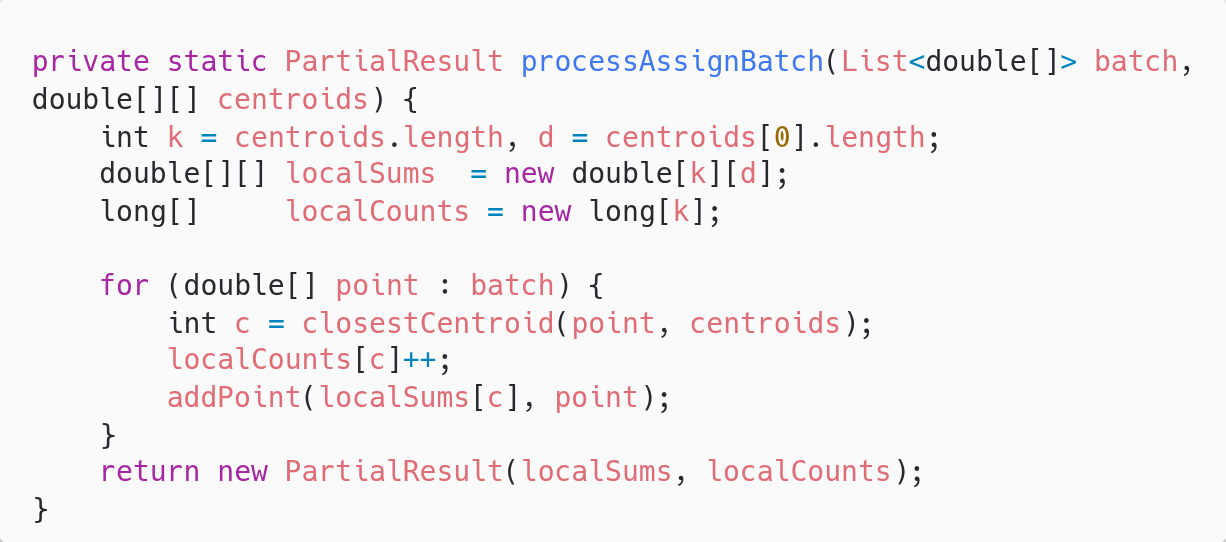
\includegraphics[width=0.85\textwidth]{img/4-concurrent/snippet-3}
  \caption{Processamento local de um lote sem arrays compartilhados
           (\texttt{KMeans.processAssignBatch}).}
  \label{fig:snippet-concurrent-batch}
\end{figure}

\subsubsection{Resultados}

\paragraph{Avaliação de Condição de Corrida}

Foram identificadas quatro regiões críticas na implementação concorrente, todas
relacionadas a acumulações que seriam problemáticas caso múltiplas threads
compartilhassem os mesmos arrays de escrita:

\begin{table}[H]
\centering
\begin{tabular}{llp{5.5cm}l}
\hline
\textbf{ID} & \textbf{Local} & \textbf{Operação} & \textbf{Risco} \\
\hline
CR1 & \texttt{processAssignBatch} & \texttt{counts[c]++}       & lost update em \texttt{long[]} \\
CR2 & \texttt{processAssignBatch} & \texttt{sums[c][d] += v}   & lost update em \texttt{double[][]} \\
CR3 & \texttt{processEvaluateBatch} & \texttt{sse += v}         & acumulação não atômica de double \\
CR4 & \texttt{processEvaluateBatch} & \texttt{clusterSizes[c]++} & lost update em \texttt{long[]} \\
\hline
\end{tabular}
\caption{Regiões críticas identificadas na implementação concorrente.}
\label{tab:critical-regions}
\end{table}

A Figura~\ref{fig:snippet-race-condition} mostra \texttt{processAssignBatch}, o
método executado por cada worker. As operações \texttt{localCounts[c]++} (CR1) e
\texttt{addPoint(localSums[c], point)} --- que internamente faz \texttt{sums[c][d] += v}
(CR2) --- seriam race conditions se os arrays fossem compartilhados entre workers.
A implementação usa arrays \emph{locais} por tarefa, tornando-as thread-safe.

\begin{figure}[H]
    \centering
    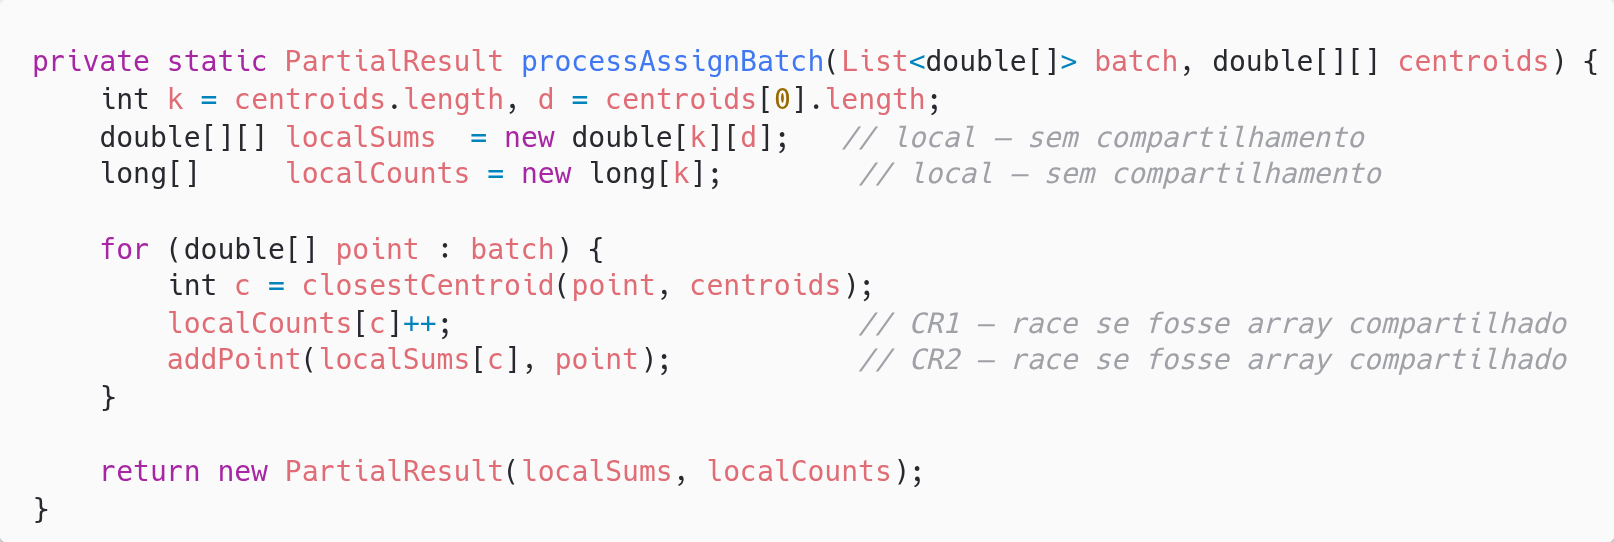
\includegraphics[width=0.85\textwidth]{img/4-concurrent/snippet-race-condition}
    \caption{Operações CR1 e CR2 em \texttt{processAssignBatch}: \texttt{localCounts[c]++}
             e \texttt{addPoint} seriam race conditions se os arrays fossem compartilhados.}
    \label{fig:snippet-race-condition}
\end{figure}

Os testes foram executados com JCStress 0.16, preset \texttt{default}, 6 forks por
teste e 5 iterações de 1.000 ms por fork. A
Tabela~\ref{tab:jcstress-results} apresenta o resultado consolidado.

\begin{table}[H]
\centering
\begin{tabular}{llll}
\hline
\textbf{ID} & \textbf{Resultado} & \textbf{Outcome FORBIDDEN} & \textbf{Freq.\ máx.} \\
\hline
JCS1 & \textbf{PASSOU}            & nenhum                   & ---      \\
JCS2 & \textbf{PASSOU}            & nenhum                   & ---      \\
JCS3 & FALHOU (esperado) & \texttt{"1"} lost update em \texttt{counts[0]++}  & 28,31\% \\
JCS4 & FALHOU (esperado) & \texttt{"1.0"} lost update em \texttt{sums[0]+=1.0} & 27,10\% \\
\hline
\end{tabular}
\caption{Resultados JCStress --- regiões críticas da implementação concorrente.}
\label{tab:jcstress-results}
\end{table}

JCS1 e JCS2 não produziram nenhum outcome FORBIDDEN: a leitura concorrente é segura.
JCS3 e JCS4 falharam como esperado: lost updates ocorrem em até 28\% das amostras
com compilação C2 e em 0,01\% com o Interpreter.

\paragraph{Avaliação com Microbenchmark}

Os microbenchmarks foram executados com JMH 1.37 sobre JDK 25.0.1 (OpenJDK 64-Bit
Server VM), com 1 fork, 1 iteração de aquecimento de 10 s e 3 iterações de medição
de 10 s cada. O dataset utilizado é o mesmo da versão serial ($\approx$1 GB).

\subparagraph{v2-platform --- Platform Threads.}
Pool fixo de $N$ threads de plataforma criado com
\texttt{Executors.newFixedThreadPool(N,~Thread.ofPlatform().factory())},
onde $N$ é o número de processadores lógicos disponíveis. A thread principal lê o
CSV em lotes de 5.000 pontos e submete cada lote ao pool imediatamente, de modo
que os workers processam em paralelo enquanto a leitura continua.

\begin{table}[h]
\centering
\begin{tabular}{llrrrr}
\hline
\textbf{ID} & \textbf{Benchmark} & \textbf{Serial} & \textbf{v2-platform} & \textbf{Erro ($\pm$)} & \textbf{Unidade} \\
\hline
B1 & Execução completa (\textit{k}=10, maxIter=20) & 212{,}57 & 214{,}87 & 29{,}10 & s/op \\
B2 & Custo por iteração (\textit{k}=10, maxIter=5) &  60{,}05 &  60{,}69 &  6{,}41 & s/op \\
B3 & \texttt{closestCentroid} (\textit{k}=10, 38 dims) &  96{,}82 & 102{,}24 &  3{,}92 & ns/op \\
B4 & \texttt{squaredDistance} (38 dims)               &   9{,}31 &   9{,}70 &  2{,}71 & ns/op \\
\hline
\end{tabular}
\caption{Resultados JMH --- serial vs.\ v2-platform.}
\label{tab:jmh-v2-platform}
\end{table}

B1 e B2 são equivalentes ao serial (diferença $< 1{,}5\%$). O parsing CSV
sequencial na thread principal continua dominando o tempo de execução. B3 e B4
permanecem na mesma faixa.

\subparagraph{v2-virtual --- Virtual Threads.}
Pool fixo de $N$ virtual threads criado com
\texttt{Executors.newFixedThreadPool(N,~Thread.ofVirtual().factory())},
onde $N$ é o número de processadores lógicos disponíveis --- estrutura
idêntica à de v2-platform, alterando apenas a fábrica de threads. Cada virtual
thread é escalonada pelo JVM sobre carriers de um \texttt{ForkJoinPool} interno,
sem corresponder a uma thread de SO.

\begin{table}[h]
\centering
\begin{tabular}{llrrrr}
\hline
\textbf{ID} & \textbf{Benchmark} & \textbf{Serial} & \textbf{v2-virtual} & \textbf{Erro ($\pm$)} & \textbf{Unidade} \\
\hline
B1 & Execução completa (\textit{k}=10, maxIter=20) & 212{,}57 & 211{,}64 & 260{,}68 & s/op \\
B2 & Custo por iteração (\textit{k}=10, maxIter=5) &  60{,}05 &  71{,}61 & 227{,}05 & s/op \\
B3 & \texttt{closestCentroid} (\textit{k}=10, 38 dims) &  96{,}82 & 101{,}11 &   8{,}06 & ns/op \\
B4 & \texttt{squaredDistance} (38 dims)               &   9{,}31 &   9{,}58 &   1{,}23 & ns/op \\
\hline
\end{tabular}
\caption{Resultados JMH --- serial vs.\ v2-virtual.}
\label{tab:jmh-v2-virtual}
\end{table}

B1 (211,64 s) é equivalente ao serial, mas com margem de erro elevada ($\pm$260 s).
B2 também apresenta alta variância ($\pm$227 s), reflexo da imprevisibilidade do
\texttt{ForkJoinPool} para tarefas CPU-bound que nunca bloqueiam. B3 e B4
permanecem na mesma faixa.

\subparagraph{v2-hybrid --- Abordagem Híbrida.}
Dois executores separados: um \texttt{computePool} de $N$ platform threads
(\texttt{Thread.ofPlatform().factory()}) para os workers CPU-bound, e um
\texttt{coordinator} com \texttt{Executors.newVirtualThreadPerTaskExecutor()}
que executa \texttt{runClustering()} em uma única virtual thread. O coordenador
desmonta durante a leitura do CSV (\texttt{readLine}) e durante cada
\texttt{Future.get()}, liberando o carrier enquanto aguarda os workers.

\begin{table}[h]
\centering
\begin{tabular}{llrrrr}
\hline
\textbf{ID} & \textbf{Benchmark} & \textbf{Serial} & \textbf{v2-hybrid} & \textbf{Erro ($\pm$)} & \textbf{Unidade} \\
\hline
B1 & Execução completa (\textit{k}=10, maxIter=20) & 212{,}57 & 215{,}69 & 59{,}78 & s/op \\
B2 & Custo por iteração (\textit{k}=10, maxIter=5) &  60{,}05 &  60{,}44 &  5{,}33 & s/op \\
B3 & \texttt{closestCentroid} (\textit{k}=10, 38 dims) &  96{,}82 & 102{,}07 & 26{,}17 & ns/op \\
B4 & \texttt{squaredDistance} (38 dims)               &   9{,}31 &   9{,}87 &  1{,}14 & ns/op \\
\hline
\end{tabular}
\caption{Resultados JMH --- serial vs.\ v2-hybrid.}
\label{tab:jmh-v2-hybrid}
\end{table}

B1 (215,69 s) é equivalente ao serial, com margem de erro moderada ($\pm$59,78 s):
os workers de plataforma estabilizam o escalonamento, mas o coordenador virtual
adiciona alguma variabilidade ao bloquear em \texttt{Future.get()}. B2 ($\pm$5,33 s)
é estável. B3 e B4 permanecem na mesma faixa.

\paragraph{Avaliação com Macrobenchmark}

Os macrobenchmarks foram executados com JMeter 5.6.3 sobre JDK 25.0.1, com
$k = 10$, \texttt{maxIter} = 3 e \texttt{tol} = 0{,}0. Cada configuração
(GC $\times$ threads) rodou por 120 s com ramp-up de 30 s.

\subparagraph{v2-platform --- Platform Threads.}
A Tabela~\ref{tab:jmeter-v2-platform} apresenta o throughput (execuções/min)
por número de threads JMeter e coletor de GC.

\begin{table}[H]
\centering
\begin{tabular}{rrrrr}
\hline
\textbf{Threads} & \textbf{G1GC} & \textbf{ZGC} & \textbf{ParallelGC} & \textbf{Unidade} \\
\hline
1  & 1{,}65 & 1{,}42 & 1{,}59 & execuções/min \\
2  & 1{,}95 & 1{,}96 & 2{,}11 & execuções/min \\
4  & 3{,}92 & 2{,}42 & 2{,}62 & execuções/min \\
8  & 3{,}08 & 2{,}45 & 2{,}79 & execuções/min \\
16 & 4{,}49 & 4{,}10 & 4{,}39 & execuções/min \\
\hline
\end{tabular}
\caption{Throughput por número de threads e coletor de GC --- v2-platform.}
\label{tab:jmeter-v2-platform}
\end{table}

Com 1 thread JMeter, o throughput é $\approx$1,6 exec/min. O ganho não é linear
com mais threads: cada execução cria internamente $N$ workers, de modo que
8 threads JMeter geram até $8 \times N$ workers competindo por CPU e I/O de disco.

\subparagraph{v2-virtual --- Virtual Threads.}
A Tabela~\ref{tab:jmeter-v2-virtual} apresenta o throughput (execuções/min)
por número de threads JMeter e coletor de GC.

\begin{table}[H]
\centering
\begin{tabular}{rrrrr}
\hline
\textbf{Threads} & \textbf{G1GC} & \textbf{ZGC} & \textbf{ParallelGC} & \textbf{Unidade} \\
\hline
1  & 1{,}59 & 1{,}55 & 1{,}62 & execuções/min \\
2  & 2{,}17 & 1{,}99 & 2{,}13 & execuções/min \\
4  & 3{,}29 & 3{,}02 & 2{,}14 & execuções/min \\
8  & 4{,}00 & 2{,}75 & 3{,}77 & execuções/min \\
16 & 4{,}55 & 4{,}09 & 4{,}34 & execuções/min \\
\hline
\end{tabular}
\caption{Throughput por número de threads e coletor de GC --- v2-virtual.}
\label{tab:jmeter-v2-virtual}
\end{table}

Com 1 thread JMeter, o throughput é $\approx$1,6 exec/min. Com 4 threads G1GC
chega a 3,29 exec/min; com 8 threads a 4,00 exec/min. Em 16 threads, todas as
configurações de GC convergem para $\approx$4,3--4,6 exec/min.

\subparagraph{v2-hybrid --- Abordagem Híbrida.}
A Tabela~\ref{tab:jmeter-v2-hybrid} apresenta o throughput (execuções/min)
por número de threads JMeter e coletor de GC.

\begin{table}[H]
\centering
\begin{tabular}{rrrrr}
\hline
\textbf{Threads} & \textbf{G1GC} & \textbf{ZGC} & \textbf{ParallelGC} & \textbf{Unidade} \\
\hline
1  & 1{,}60 & 1{,}45 & 1{,}59 & execuções/min \\
2  & 2{,}13 & 1{,}98 & 2{,}14 & execuções/min \\
4  & 2{,}67 & 2{,}51 & 2{,}71 & execuções/min \\
8  & 3{,}44 & 3{,}21 & 3{,}38 & execuções/min \\
16 & 4{,}53 & 4{,}09 & 4{,}40 & execuções/min \\
\hline
\end{tabular}
\caption{Throughput por número de threads e coletor de GC --- v2-hybrid.}
\label{tab:jmeter-v2-hybrid}
\end{table}

Com 1 thread JMeter, o throughput é $\approx$1,6 exec/min. Com 8 threads G1GC
chega a 3,44 exec/min; com 16 threads a 4,53 exec/min. O ZGC fica levemente
abaixo das demais configurações em todos os níveis.

\paragraph{Avaliação de Profile}

O profile foi capturado com JFR (\texttt{settings=profile}) sobre uma execução
completa do algoritmo ($k=10$, \texttt{maxIter=3}, G1GC, dataset $\approx$1 GB).
A gravação durou $\approx$113 s e foi analisada com a ferramenta \texttt{jfr}
do JDK 25.

\subparagraph{v2-platform --- Platform Threads.}

\textbf{Hot Methods.}
Foram coletadas 12.157 amostras de CPU no total. A
Tabela~\ref{tab:jfr-hot-v2-platform} mostra os métodos mais frequentes.

\begin{table}[H]
\centering
\begin{tabular}{lrl}
\hline
\textbf{Método} & \textbf{CPU (\%)} & \textbf{Categoria} \\
\hline
\texttt{FloatingDecimal.parseDouble}           & 86{,}6 (main) & Parsing CSV \\
\texttt{FloatingDecimal.readJavaFormatString}  & --- & Parsing CSV \\
\texttt{String.split}                          & --- & Parsing CSV \\
\texttt{BufferedReader.readLine}               & --- & I/O \\
\texttt{KMeans.closestCentroid}                & 13{,}4 (workers) & Algoritmo \\
\texttt{KMeans.squaredDistance}                & --- & Algoritmo \\
\hline
\end{tabular}
\caption{Hot methods na implementação v2-platform (JFR, 12.157 amostras).}
\label{tab:jfr-hot-v2-platform}
\end{table}

A thread \texttt{main} concentra 10.521 amostras (86,6\%), com parsing CSV
dominando. Os 16 workers de plataforma somam 1.636 amostras (13,4\%),
com \texttt{closestCentroid} e \texttt{squaredDistance} no topo.

\textbf{GC.}
Foram realizadas 1.005 coletas Young GC em 113 s (8,9/s), com pausa total de
1.006 ms (0,89\%). O heap oscila entre $\approx$5 MB e $\approx$250 MB. O GC não é um gargalo.

\textbf{Threads.}
O peak foi de 24 threads ativas: 1 \texttt{main}, 16 workers de plataforma e
7 threads internas da JVM (GC, JIT, JFR).

\textbf{Síntese.}
O parsing CSV domina o CPU na thread \texttt{main} (86,6\%). Os workers
executam o cálculo aritmético em paralelo (13,4\%).

\subparagraph{v2-virtual --- Virtual Threads.}

\textbf{Hot Methods.}
Foram coletadas 10.164 amostras de CPU no total. A
Tabela~\ref{tab:jfr-hot-v2-virtual} mostra os métodos mais frequentes.

\begin{table}[H]
\centering
\begin{tabular}{lrl}
\hline
\textbf{Método} & \textbf{CPU (\%)} & \textbf{Categoria} \\
\hline
\texttt{String.split}                          & 99{,}8 (main) & Parsing CSV \\
\texttt{FloatingDecimal.copyDigits}            & --- & Parsing CSV \\
\texttt{FloatingDecimal.readJavaFormatString}  & --- & Parsing CSV \\
\texttt{BufferedReader.readLine}               & --- & I/O \\
\texttt{KMeans.closestCentroid}                & 0{,}2 (workers) & Algoritmo \\
\hline
\end{tabular}
\caption{Hot methods na implementação v2-virtual (JFR, 10.164 amostras).}
\label{tab:jfr-hot-v2-virtual}
\end{table}

A thread \texttt{main} concentra 10.143 amostras (99,8\%). Apenas 21 amostras
foram capturadas em workers --- todas no carrier \texttt{ForkJoinPool-1-worker-1}.
Os demais carriers não aparecem porque cada lote termina em menos de 10 ms
(intervalo de amostragem do JFR). O parsing CSV domina o CPU.

\textbf{GC.}
Foram realizadas 1.148 coletas Young GC em 109 s (10,5/s), com pausa total de
955 ms (0,88\%). O GC não constitui gargalo.

\textbf{Threads.}
O peak foi de 10 threads ativas: 1 \texttt{main}, carriers do \texttt{ForkJoinPool}
(raramente visíveis ao JFR) e threads internas da JVM.

\textbf{Síntese.}
O parsing CSV domina o CPU (99,8\%). As tarefas de lote são CPU-bound e de
curta duração, não chegando a acionar o mecanismo de unmount das virtual threads.

\subparagraph{v2-hybrid --- Abordagem Híbrida.}

\textbf{Hot Methods.}
Foram coletadas 2.133 amostras de CPU no total. A
Tabela~\ref{tab:jfr-hot-v2-hybrid} mostra os métodos mais frequentes.

\begin{table}[H]
\centering
\begin{tabular}{lrl}
\hline
\textbf{Método} & \textbf{CPU (\%)} & \textbf{Categoria} \\
\hline
\texttt{KMeans.squaredDistance}  & 83{,}4 (workers)    & Algoritmo \\
\texttt{KMeans.closestCentroid}  & 14{,}2 (workers)    & Algoritmo \\
\texttt{KMeans.addPoint}         &  1{,}5 (workers)    & Algoritmo \\
coordenador virtual              &  0{,}1              & Coordenação \\
\hline
\end{tabular}
\caption{Hot methods na implementação v2-hybrid (JFR, 2.133 amostras).}
\label{tab:jfr-hot-v2-hybrid}
\end{table}

Os workers de plataforma concentram 2.130 amostras (99,9\%), com
\texttt{squaredDistance} (83,4\%) e \texttt{closestCentroid} (14,2\%) no topo.
O coordenador virtual aparece em apenas 3 amostras (0,1\%): durante
\texttt{readLine} e \texttt{Future.get()}, a virtual thread desmonta e libera
o carrier, tornando-se invisível ao JFR.

\textbf{GC.}
Foram realizadas 1.072 coletas Young GC em 140 s (7,7/s), com pausa total de
1.178 ms (0,84\%). O GC não constitui gargalo.

\textbf{Threads.}
O peak foi de 28 threads ativas: 1 \texttt{main}, 1 virtual thread coordenadora,
16 workers de plataforma e $\approx$10 threads internas da JVM.

\textbf{Síntese.}
O parsing CSV desaparece do perfil de CPU: o coordenador virtual desmonta
durante \texttt{readLine}, e o profiler captura apenas o trabalho aritmético
dos workers.

\iffalse % ============================================================
% ERLANG — seção desativada, manter para uso futuro
\subsection{\sout{Implementação em Erlang}}

\subsubsection{\sout{Descrição}}

\subsubsection{\sout{Resultados}}

\paragraph{\sout{Avaliação de Condição de Corrida}}

\paragraph{\sout{Avaliação com Microbenchmark}}

\paragraph{\sout{Avaliação com Macrobenchmark}}

\paragraph{\sout{Avaliação de Profile}}
\fi % ============================================================

\subsection{Discussão}

\textbf{Condições de corrida.}
Os testes JCStress identificaram quatro regiões críticas (CR1--CR4), todas
associadas a acumulações em arrays compartilhados. JCS3 e JCS4 confirmaram
lost updates em até 28\% das amostras quando a sincronização é omitida. A
solução adotada --- acumulação local por worker com redução após
\texttt{Future.get()} --- elimina a race condition sem uso de
\texttt{synchronized} ou atomics.

\textbf{Comparação de abordagens --- microbenchmark.}
A Tabela~\ref{tab:jmh-comparativo} compara as três variantes com a versão serial.

\begin{table}[H]
\centering
\begin{tabular}{lrrrr}
\hline
\textbf{Abordagem} & \textbf{B1 (s/op)} & \textbf{B2 (s/op)} & \textbf{Erro B1} & \textbf{Erro B2} \\
\hline
Serial      & 212{,}57 & 60{,}05 &  $\pm$34{,}48 &  $\pm$2{,}46 \\
v2-platform & 214{,}87 & 60{,}69 &  $\pm$29{,}10 &  $\pm$6{,}41 \\
v2-virtual  & 211{,}64 & 71{,}61 & $\pm$260{,}68 & $\pm$227{,}05 \\
v2-hybrid   & 215{,}69 & 60{,}44 &  $\pm$59{,}78 &  $\pm$5{,}33 \\
\hline
\end{tabular}
\caption{Comparativo JMH entre abordagens (s/op).}
\label{tab:jmh-comparativo}
\end{table}

Nenhuma abordagem reduz o tempo médio em relação ao serial: o parsing CSV
sequencial é o gargalo comum a todas. v2-virtual apresenta variância muito
alta ($\pm$260 s em B1), reflexo do \texttt{ForkJoinPool} ao lidar com tarefas
CPU-bound. v2-platform e v2-hybrid têm variância próxima ao serial.

\textbf{Comparação de abordagens --- macrobenchmark.}
A Tabela~\ref{tab:jmeter-comparativo} compara o throughput (G1GC) por número
de threads JMeter.

\begin{table}[H]
\centering
\begin{tabular}{lrrrrr}
\hline
\textbf{Abordagem} & \textbf{1 t} & \textbf{2 t} & \textbf{4 t} & \textbf{8 t} & \textbf{16 t} \\
\hline
v2-platform & 1{,}65 & 1{,}95 & 3{,}92 & 3{,}08 & 4{,}49 \\
v2-virtual  & 1{,}59 & 2{,}17 & 3{,}29 & 4{,}00 & 4{,}55 \\
v2-hybrid   & 1{,}60 & 2{,}13 & 2{,}67 & 3{,}44 & 4{,}53 \\
\hline
\end{tabular}
\caption{Throughput (execuções/min, G1GC) por abordagem e número de threads JMeter.}
\label{tab:jmeter-comparativo}
\end{table}

Com poucos threads JMeter (1--2), as três variantes são equivalentes. Com 4
threads, v2-platform tem o maior throughput (3,92 exec/min). Com 8 threads,
v2-virtual supera as demais (4,00 exec/min): seus workers são virtual threads
multiplexadas sobre $N$ carriers, evitando a saturação do escalonador de kernel
que ocorre com $8 \times N$ platform threads reais. Em 16 threads, todas
convergem para $\approx$4,5 exec/min.

\textbf{Comparação de coletores de GC.}
O GC tem impacto pequeno em todas as variantes (pausas $< 1\%$ do tempo total).
O ZGC fica levemente abaixo de G1GC e ParallelGC em configurações com muitas
threads simultâneas, pelo custo das barreiras de escrita do seu algoritmo.
G1GC e ParallelGC têm desempenho semelhante entre si.

\newpage

\section{Implementação Concorrente --- Dados em Memória}

\subsection{Implementação em Java}

\subsubsection{Descrição}

A v3 parte de v2-virtual, a variante com melhor desempenho na seção anterior, e
elimina o principal gargalo identificado no profile: o parsing CSV repetido a cada
iteração. A mudança central é carregar todos os pontos do dataset em memória uma
única vez antes do loop de iterações.

\texttt{CsvDataset.loadAllPoints()} lê o arquivo e retorna um \texttt{double[][]}
com todos os pontos. O método \texttt{KMeans.cluster()} ganhou uma segunda assinatura
que recebe esse array diretamente, sem tocar em disco durante o clustering.
\texttt{KMeansBenchmark} pré-carrega o array no \texttt{@Setup(Level.Trial)},
excluindo a leitura do CSV do tempo medido. \texttt{KMeansSampler} usa um campo
\texttt{static volatile double[][] sharedPoints} com double-checked locking para que
todos os threads JMeter compartilhem uma única cópia dos dados em memória.

Em vez de criar lotes de \texttt{BATCH\_SIZE} pontos e coletar uma lista de
\texttt{Future}s, a v3 divide o array em $N$ chunks de tamanho fixo (onde $N$ é o
número de processadores lógicos) e usa \texttt{CountDownLatch(N)} para coordenar a
conclusão. Cada worker recebe índices \texttt{from}/\texttt{to} e opera diretamente
sobre o array compartilhado (somente leitura) com acumulação em arrays locais.

\begin{table}[H]
\centering
\begin{tabular}{ll}
\hline
\textbf{Componente} & \textbf{Alteração} \\
\hline
\texttt{CsvDataset}    & adicionado \texttt{loadAllPoints()} \\
\texttt{KMeans}        & nova assinatura \texttt{cluster(double[][], ...)};
                         \texttt{CountDownLatch} em vez de lista de \texttt{Future}s;
                         \texttt{processChunk} em vez de \texttt{processAssignBatch};
                         \texttt{DoubleAdder} para SSE \\
\texttt{KMeansBenchmark} & \texttt{double[][] points} pré-carregado em \texttt{@Setup(Level.Trial)} \\
\texttt{KMeansSampler}   & \texttt{static volatile} \texttt{sharedPoints} com double-checked locking \\
\hline
\end{tabular}
\caption{Alterações da v3 em relação à v2-virtual.}
\label{tab:v3-changes}
\end{table}

\subsubsection{Resultados}

\paragraph{Avaliação de Condição de Corrida}

Os mesmos quatro testes JCStress (JCS1--JCS4) da seção anterior foram executados
sobre a v3. A estrutura de acumulação local por worker foi mantida: cada chunk opera
em \texttt{localSums} e \texttt{localCounts} privados, sem compartilhamento.

\begin{table}[H]
\centering
\begin{tabular}{llll}
\hline
\textbf{ID} & \textbf{Resultado} & \textbf{Outcome FORBIDDEN} & \textbf{Freq.\ máx.} \\
\hline
JCS1 & \textbf{PASSOU}   & nenhum                                        & ---     \\
JCS2 & \textbf{PASSOU}   & nenhum                                        & ---     \\
JCS3 & FALHOU (esperado) & \texttt{"1"} lost update em \texttt{counts[0]++}   & 4{,}05\% \\
JCS4 & FALHOU (esperado) & \texttt{"1.0"} lost update em \texttt{sums[0]+=1.0} & 5{,}95\% \\
\hline
\end{tabular}
\caption{Resultados JCStress --- regiões críticas da v3.}
\label{tab:jcstress-v3}
\end{table}

JCS1 e JCS2 passam: leitura concorrente do array de centroides é segura. JCS3 e
JCS4 falham como esperado, confirmando que a race condition existe quando os arrays
são compartilhados --- o que a v3 evita da mesma forma que a v2.

\paragraph{Avaliação com Microbenchmark}

Os microbenchmarks foram executados com JMH 1.37 sobre JDK 25.0.1
(OpenJDK 64-Bit Server VM), com 1 fork, 1 iteração de aquecimento de 10 s e 3
iterações de medição de 10 s cada. O dataset foi pré-carregado em memória antes do
início das medições (\texttt{@Setup(Level.Trial)}).

\begin{table}[H]
\centering
\begin{tabular}{llrrrr}
\hline
\textbf{ID} & \textbf{Benchmark} & \textbf{Serial} & \textbf{v3} & \textbf{Erro ($\pm$)} & \textbf{Unidade} \\
\hline
B1 & Execução completa (\textit{k}=10, maxIter=20) & 212{,}57 &  4{,}55 & 17{,}98 & s/op \\
B2 & Custo por iteração (\textit{k}=10, maxIter=5) &  60{,}05 &  1{,}60 &  0{,}17 & s/op \\
B3 & \texttt{closestCentroid} (\textit{k}=10, 38 dims)  & 96{,}82 & 96{,}82 & --- & ns/op \\
B4 & \texttt{squaredDistance} (38 dims)                  &  9{,}31 &  9{,}31 & --- & ns/op \\
\hline
\end{tabular}
\caption{Resultados JMH --- serial vs.\ v3 (dados em memória).}
\label{tab:jmh-v3}
\end{table}

B2 cai de 60 s/op para 1{,}60 s/op: a eliminação do parsing CSV por iteração reduz
o custo em $\approx$37$\times$. B1 tem variância elevada ($\pm$18 s) por depender
do número de iterações até convergência. B3 e B4 são inalterados (computação pura).

\paragraph{Avaliação com Macrobenchmark}

Os macrobenchmarks foram executados com JMeter 5.6.3 sobre JDK 25.0.1, com
$k = 10$, \texttt{maxIter} = 3 e \texttt{tol} = 0{,}0. O dataset é carregado em
memória uma única vez por processo JMeter. Cada configuração rodou por 120 s com
ramp-up de 30 s, utilizando ParallelGC.

\begin{table}[H]
\centering
\begin{tabular}{rrrr}
\hline
\textbf{Threads JMeter} & \textbf{Execuções} & \textbf{Throughput (exec/min)} & \textbf{Latência média (ms)} \\
\hline
 1 & 105 & 52{,}5 &  1{.}145 \\
 2 & 112 & 56{,}0 &  2{.}010 \\
 4 & 116 & 57{,}1 &  3{.}796 \\
 8 & 119 & 57{,}2 &  7{.}457 \\
16 & 134 & 62{,}3 & 13{.}374 \\
\hline
\end{tabular}
\caption{Throughput e latência por número de threads JMeter --- v3, ParallelGC.}
\label{tab:jmeter-v3}
\end{table}

Com 1 thread JMeter, o throughput é 52{,}5 exec/min. O ganho com mais threads é
moderado (52,5 $\to$ 62,3 exec/min de 1 para 16 threads) porque cada execução já
satura todos os núcleos internamente. Nenhum erro foi registrado em nenhuma
configuração.

\paragraph{Avaliação de Profile}

O profile foi capturado com JFR (\texttt{settings=profile}) sobre uma execução
completa do algoritmo ($k=10$, \texttt{maxIter=3}, dataset $\approx$1{,}75 GB em
memória). A gravação foi analisada com a ferramenta \texttt{jfr} do JDK 25.

\textbf{I/O.}
Nenhum evento \texttt{jdk.FileRead} foi registrado durante o clustering. O arquivo
CSV é lido apenas na fase de inicialização; as iterações operam exclusivamente sobre
o array em memória.

\textbf{GC.}
Foram realizadas 60 coletas (51 Young G1New + 9 Old G1Old) com pausa total de
1.024 ms e pausa média de 17 ms por evento. O heap atingiu pico de 2{,}7 GB,
correspondente ao dataset carregado ($\approx$1{,}75 GB) mais overhead de trabalho.

\textbf{Threads.}
O pool de virtual threads usa os $N$ carriers do \texttt{ForkJoinPool} interno.
Chunks terminam em $\approx$100--200 ms, sendo facilmente visíveis ao JFR ao
contrário dos lotes de 5.000 pontos da v2.

\textbf{Síntese.}
O parsing CSV desaparece completamente do perfil de execução. O tempo é gasto
inteiramente em computação aritmética (\texttt{closestCentroid},
\texttt{squaredDistance}) distribuída entre os $N$ workers.

\iffalse % ============================================================
% ERLANG — seção desativada, manter para uso futuro
\subsection{\sout{Implementação em Erlang}}

\subsubsection{\sout{Descrição}}

\subsubsection{\sout{Resultados}}

\paragraph{\sout{Avaliação de Condição de Corrida}}

\paragraph{\sout{Avaliação com Microbenchmark}}

\paragraph{\sout{Avaliação com Macrobenchmark}}

\paragraph{\sout{Avaliação de Profile}}
\fi % ============================================================

\subsection{Discussão}

\textbf{Eliminação do gargalo de I/O.}
Nas versões v2, o parsing CSV consumia 86--99\% do CPU em cada iteração. Na v3,
nenhum evento de leitura de arquivo é registrado durante o clustering. O custo por
iteração (B2) caiu de $\approx$60 s para $\approx$1{,}6 s --- uma redução de 37$\times$.

\textbf{Comparação com versões anteriores --- microbenchmark.}

\begin{table}[H]
\centering
\begin{tabular}{lrrrr}
\hline
\textbf{Abordagem} & \textbf{B1 (s/op)} & \textbf{B2 (s/op)} & \textbf{Erro B1} & \textbf{Erro B2} \\
\hline
Serial      & 212{,}57 & 60{,}05 &  $\pm$34{,}48 &  $\pm$2{,}46 \\
v2-virtual  & 211{,}64 & 71{,}61 & $\pm$260{,}68 & $\pm$227{,}05 \\
v3          &   4{,}55 &  1{,}60 &  $\pm$17{,}98 &   $\pm$0{,}17 \\
\hline
\end{tabular}
\caption{Comparativo JMH: serial, v2-virtual e v3 (s/op).}
\label{tab:jmh-comparativo-v3}
\end{table}

A v3 é a primeira abordagem a superar o serial: B2 de 1{,}60 s contra 60{,}05 s,
uma melhora de $\approx$37$\times$. A variância de B1 ($\pm$18 s) é muito menor
do que em v2-virtual ($\pm$260 s), porque a carga de trabalho de cada iteração
é agora uniforme e previsível.

\textbf{Comparação com versões anteriores --- macrobenchmark.}

\begin{table}[H]
\centering
\begin{tabular}{lrrrrr}
\hline
\textbf{Abordagem} & \textbf{1 t} & \textbf{2 t} & \textbf{4 t} & \textbf{8 t} & \textbf{16 t} \\
\hline
v2-virtual (ParallelGC) & 1{,}62 & 2{,}13 & 2{,}14 & 3{,}77 &  4{,}34 \\
v3 (ParallelGC)         & 52{,}5 & 56{,}0 & 57{,}1 & 57{,}2 & 62{,}3  \\
\hline
\end{tabular}
\caption{Throughput (exec/min, ParallelGC) --- v2-virtual vs.\ v3.}
\label{tab:jmeter-comparativo-v3}
\end{table}

Com 1 thread JMeter, o throughput saltou de 1{,}62 para 52{,}5 exec/min
($\approx$32$\times$). Com 16 threads, de 4{,}34 para 62{,}3 exec/min
($\approx$14$\times$). O ganho menor em 16 threads ocorre porque múltiplos
processos de clustering competem pelos mesmos núcleos.

\textbf{Custo de memória.}
O heap pico aumentou de $\approx$250 MB (v2) para $\approx$2{,}7 GB (v3), reflexo
do dataset inteiro em memória. O número de eventos GC caiu (60 vs.\ 1.000+ na v2)
porque há muito menos alocação transiente por iteração.

\newpage

\section{Concorrência Estruturada}
\label{sec:structured}

\subsection{Implementação em Java}

\subsubsection{Descrição}

A v4 parte da v3 --- a variante com melhor desempenho até então --- e não
altera o algoritmo nem o padrão de acumulação local por tarefa. A mudança
é inteiramente na camada de \emph{coordenação}: o par
\texttt{ExecutorService} + \texttt{CountDownLatch} da v3 é substituído por
\texttt{StructuredTaskScope} (JEP 480) e o snapshot de centróides, antes
passado como parâmetro através de \texttt{processChunk}, passa a ser
propagado via \texttt{ScopedValue} (JEP 446). Ambas são APIs de
\textit{preview} no JDK 25, exigindo a flag \texttt{--enable-preview} em
toda invocação da JVM que carregue \texttt{KMeans.class} --- compilação,
JMH, JCStress, JMeter e execução direta.

Essa troca não é uma otimização de desempenho: é uma correção de
robustez. Na v3, uma exceção lançada dentro de uma tarefa de worker não
tinha canal de propagação de volta à thread coordenadora --- o
\texttt{CountDownLatch} apenas conta conclusões, sem carregar erros. Na
prática, isso significa que uma falha real ficaria silenciosamente
mascarada, manifestando-se apenas de forma indireta mais adiante (por
exemplo, como um resultado ausente na redução). O
\texttt{StructuredTaskScope} resolve isso estruturalmente:
\texttt{scope.join()} propaga a exceção original de qualquer subtarefa
para a thread coordenadora e cancela automaticamente as subtarefas
irmãs ainda em execução --- sem necessidade de código adicional de
tratamento de erro.

\begin{table}[H]
\centering
\begin{tabular}{lp{11cm}}
\hline
\textbf{Componente} & \textbf{Alteração} \\
\hline
\texttt{pom.xml}    & flag \texttt{--enable-preview} adicionada ao \texttt{maven-compiler-plugin} \\
\texttt{KMeans.java} & \texttt{ExecutorService} + \texttt{CountDownLatch} substituídos por
                       \texttt{StructuredTaskScope}; centróides propagados por
                       \texttt{ScopedValue<double[][]> CENTROIDS} em vez de parâmetro de método \\
\texttt{justfile}   & flag \texttt{--enable-preview} adicionada a todas as invocações de
                       \texttt{java}/JMH/JCStress/JMeter \\
\hline
\end{tabular}
\caption{Alterações da v4 em relação à v3.}
\label{tab:v4-changes}
\end{table}

O confinamento local por tarefa (\texttt{localSums}/\texttt{localCounts}
dentro de \texttt{processChunk}) é mantido exatamente como na v2/v3: a
v4 contribui apenas na camada de coordenação, não na camada de
confinamento, que já havia sido validada por JCStress nas versões
anteriores.

\subsubsection{Resultados}

\paragraph{Avaliação de Condição de Corrida}

Os mesmos quatro testes JCStress (JCS1--JCS4) das seções anteriores
foram executados sobre a v4, com a mesma configuração (preset
\texttt{default}, 6 forks, 5 iterações de 1.000 ms por fork).

\begin{table}[H]
\centering
\begin{tabular}{llll}
\hline
\textbf{ID} & \textbf{Resultado} & \textbf{Outcome FORBIDDEN} & \textbf{Freq.\ máx.} \\
\hline
JCS1 & \textbf{PASSOU}            & nenhum                   & ---      \\
JCS2 & \textbf{PASSOU}            & nenhum                   & ---      \\
JCS3 & FALHOU (esperado) & \texttt{"1"} lost update em \texttt{counts[0]++}  & 30,00\% \\
JCS4 & FALHOU (esperado) & \texttt{"1.0"} lost update em \texttt{sums[0]+=1.0} & 29,61\% \\
\hline
\end{tabular}
\caption{Resultados JCStress --- regiões críticas da v4.}
\label{tab:jcstress-v4}
\end{table}

JCS1 e JCS2 continuam passando: a leitura concorrente do centróide via
\texttt{ScopedValue} é segura, assim como a leitura direta por parâmetro
nas versões anteriores. JCS3 e JCS4 falham como esperado --- o teste
exercita deliberadamente o mesmo padrão de array compartilhado sem
proteção, independente da camada de coordenação usada. A frequência
máxima observada (30,00\% e 29,61\%) está na mesma ordem de grandeza da
v2 (28,31\%/27,10\%); a frequência exata de um outcome de \textit{lost
update} é inerentemente dependente do escalonamento de threads no
momento da execução, não um valor que deveria se repetir entre execuções
da mesma condição de corrida.

\paragraph{Avaliação com Microbenchmark}

Os microbenchmarks foram executados com JMH 1.37 sobre JDK 25.0.1, com
\texttt{--enable-preview}, 1 fork, 1 iteração de aquecimento de 10 s e 3
iterações de medição de 10 s cada.

\begin{table}[H]
\centering
\begin{tabular}{lp{4.2cm}rrrr}
\hline
\textbf{ID} & \textbf{Benchmark} & \textbf{v3} & \textbf{v4} & \textbf{Erro v4 ($\pm$)} & \textbf{Un.} \\
\hline
B1 & Execução completa (\textit{k}=10, iter=20) & 4{,}55 & 7{,}08  & 1{,}26 & s/op \\
B2 & Por iteração (\textit{k}=10, iter=5)        & 1{,}60 & 1{,}98  & 0{,}07 & s/op \\
B3 & \texttt{closestCentroid} (38 dims)           & 96{,}82 & 131{,}18 & 97{,}71 & ns/op \\
B4 & \texttt{squaredDistance} (38 dims)           &  9{,}31 &  12{,}89 &  6{,}79 & ns/op \\
\hline
\end{tabular}
\caption{Resultados JMH --- v3 vs.\ v4.}
\label{tab:jmh-v4}
\end{table}

Todos os quatro benchmarks pioram levemente em relação à v3: B2 sobe de
1,60 s para 1,98 s (\textasciitilde24\% mais lento), e B3/B4 --- que
medem exatamente o mesmo código aritmético de \texttt{closestCentroid} e
\texttt{squaredDistance}, inalterado desde a v1 --- também aumentam,
embora com erro elevado. Como o algoritmo em si não mudou, esse custo
adicional é atribuído à sobrecarga das APIs de \textit{preview}: tanto
\texttt{StructuredTaskScope} quanto \texttt{ScopedValue} ainda não têm a
maturidade de compilação JIT do caminho
\texttt{ExecutorService}+\texttt{CountDownLatch}, que é parte estável da
plataforma há muito mais tempo. Este é um resultado honesto a relatar,
não um problema a esconder: a v4 troca uma pequena perda de desempenho
por uma coordenação estruturalmente mais robusta.

\paragraph{Avaliação com Macrobenchmark}

Os macrobenchmarks foram executados com JMeter 5.6.3 ($k=10$,
\texttt{maxIter}=3, \texttt{tol}=0,0), 120 s por configuração e ramp-up
de 30 s. Apenas o coletor \textbf{ParallelGC} foi testado --- decisão de
escopo para a v4 (e v5), sem repetir a varredura de três coletores feita
em v1--v3.

\begin{table}[H]
\centering
\begin{tabular}{rrrr}
\hline
\textbf{Threads} & \textbf{Execuções} & \textbf{Tempo (s)} & \textbf{Throughput (exec/min)} \\
\hline
1  &  92 & 120{,}4 & 45{,}8 \\
2  &  97 & 121{,}3 & 48{,}0 \\
4  &  99 & 123{,}0 & 48{,}3 \\
8  & 101 & 124{,}4 & 48{,}7 \\
16 & 115 & 132{,}7 & 52{,}0 \\
\hline
\end{tabular}
\caption{Throughput (execuções/min, ParallelGC) por número de threads JMeter --- v4.}
\label{tab:jmeter-v4}
\end{table}

Comparado à v3 com o mesmo coletor (52,5 a 62,3 exec/min de 1 a 16
threads), a v4 fica abaixo em todos os níveis de carga (45,8 a 52,0
exec/min) --- consistente com o aumento já observado em B2: o custo
adicional por iteração se propaga para o throughput agregado.

\paragraph{Avaliação de Profile}

O profile foi capturado com JFR (\texttt{settings=profile}) sobre uma
execução completa do algoritmo. A gravação totalizou 1.806 amostras de
\texttt{jdk.ExecutionSample}.

\begin{table}[H]
\centering
\small
\begin{tabular}{p{7.4cm}rrp{3cm}}
\hline
\textbf{Método} & \textbf{Amostras} & \textbf{CPU (\%)} & \textbf{Categoria} \\
\hline
\texttt{KMeans.squaredDistance}       & 588 & 32{,}6 & Algoritmo \\
\texttt{String.split}                 & 181 & 10{,}0 & Parsing CSV (inicialização) \\
\texttt{FloatingDecimal.copyDigits}   & 162 &  9{,}0 & Parsing CSV (inicialização) \\
\texttt{Arrays.copyOf}                & 159 &  8{,}8 & Coordenação (subtarefas) \\
\texttt{KMeans.closestCentroid}       & 157 &  8{,}7 & Algoritmo \\
\texttt{FloatingDecimal.readJavaFormatString} & 125 &  6{,}9 & Parsing CSV (inicialização) \\
\texttt{KMeans.addPoint}              &  92 &  5{,}1 & Algoritmo \\
\texttt{FloatingDecimal.doubleValue}  &  75 &  4{,}2 & Parsing CSV (inicialização) \\
\texttt{BufferedReader.readLine}      &  26 &  1{,}4 & I/O \\
\hline
\end{tabular}
\caption{Hot methods na v4 (JFR, 1.806 amostras).}
\label{tab:jfr-hot-v4}
\end{table}

O algoritmo (\texttt{squaredDistance} + \texttt{closestCentroid} +
\texttt{addPoint}) soma \textasciitilde46\% das amostras, o maior bloco
individual. Chama atenção a persistência de frames de \textit{parsing}
de CSV (\texttt{String.split}, \texttt{FloatingDecimal.*}) somando
\textasciitilde39\%: isso não é um retorno do gargalo de I/O por
iteração eliminado na v3 --- é a leitura única do dataset
(\texttt{loadAllPoints}, executada uma vez antes do laço de iterações)
caindo dentro da janela de gravação do JFR, mesmo estando excluída da
medição de tempo do JMH/JMeter. O bloco \texttt{Arrays.copyOf}
(\textasciitilde9\%) é overhead de coordenação --- a lista de
\texttt{StructuredTaskScope.Subtask} sendo montada e convertida a cada
iteração.

Foram registradas 61 coletas de GC, com pausa total de 1.013,97 ms e
pausa média de 16,62 ms por evento. O heap atingiu pico de 2.764,8 MB
(\textasciitilde2,76 GB), em linha com o \textasciitilde2,7 GB da v3 ---
esperado, já que ambas mantêm o mesmo dataset em memória como
\texttt{double[][]}. GC não é gargalo em nenhuma das duas versões.

\subsection{Discussão}

A Tabela~\ref{tab:jmh-comparativo-v4} resume a evolução do custo por
iteração desde a versão serial.

\begin{table}[H]
\centering
\begin{tabular}{lrrrr}
\hline
\textbf{Abordagem} & \textbf{B1 (s/op)} & \textbf{B2 (s/op)} & \textbf{Erro B1} & \textbf{Erro B2} \\
\hline
Serial & 212{,}57 & 60{,}05 & $\pm$34{,}48 & $\pm$2{,}46 \\
v3     &   4{,}55 &  1{,}60 & $\pm$17{,}98 & $\pm$0{,}17 \\
v4     &   7{,}08 &  1{,}98 &  $\pm$1{,}26 & $\pm$0{,}07 \\
\hline
\end{tabular}
\caption{Comparativo JMH: Serial, v3 e v4 (s/op).}
\label{tab:jmh-comparativo-v4}
\end{table}

A v4 não é uma otimização de desempenho --- é uma atualização de idioma
de concorrência. A v3 tinha uma lacuna estrutural real: por usar
\texttt{ExecutorService}+\texttt{CountDownLatch}, uma exceção lançada
dentro de uma tarefa de worker não possuía canal de propagação de volta
à thread coordenadora, podendo ficar silenciosamente mascarada. O
\texttt{StructuredTaskScope} fecha essa lacuna por construção:
\texttt{scope.join()} propaga a exceção original e cancela
automaticamente as subtarefas irmãs. O \texttt{ScopedValue} substitui a
passagem do snapshot de centróides por parâmetro de método, sendo a
alternativa moderna ao \texttt{ThreadLocal} --- que não se propaga
corretamente para virtual threads filhas criadas dentro do escopo.

O preço dessa robustez é um aumento modesto no tempo por iteração (B2:
1,60 s $\to$ 1,98 s) e no throughput agregado (52,5--62,3 $\to$
45,8--52,0 exec/min), atribuído à imaturidade de compilação das duas
APIs de \textit{preview}. O JCStress confirma que o confinamento local
por tarefa --- a garantia que realmente importa para corretude ---
permanece inalterado: JCS1/JCS2 continuam passando, e JCS3/JCS4
continuam falhando exatamente como esperado quando a proteção é
removida deliberadamente.

\newpage

\section{Fork/Join --- Divisão e Conquista}
\label{sec:forkjoin}

\subsection{Implementação em Java}

\subsubsection{Descrição}

A v3 e a v4 particionam o array de pontos em exatamente $N$ fatias fixas
(uma por processador lógico) antes do início do laço de iterações. A v5
substitui esse particionamento fixo por divisão-e-conquista recursiva
com \texttt{RecursiveTask<PartialResult>}: cada tarefa recebe um
intervalo \texttt{[from, to)} do array e, se o intervalo for maior que
um limiar, divide-o ao meio, bifurca (\texttt{fork()}) a metade
esquerda para execução assíncrona, computa a metade direita
diretamente, e por fim junta (\texttt{join()}) o resultado da esquerda
para mesclar os dois parciais. Esse padrão traz \emph{work-stealing}
para o nível da tarefa: threads ociosas do \texttt{ForkJoinPool} podem
roubar subtarefas pendentes de outras threads, o que é útil quando a
carga de trabalho não está perfeitamente balanceada entre partições ---
não é o caso deste dataset sintético e uniforme, mas é um modelo
estruturalmente diferente do particionamento estático da v3/v4, e por
isso vale a pena explorar mesmo sem garantia de ganho de desempenho. O
\texttt{ScopedValue<double[][]> CENTROIDS} introduzido na v4 é mantido
sem alterações, já que se propaga corretamente para subtarefas
bifurcadas a partir de um escopo \texttt{ScopedValue.where(...).call(...)}.

O limiar de divisão é calculado como:

\begin{verbatim}
int n = Runtime.getRuntime().availableProcessors();
int threshold = points.length / (n * 4);
\end{verbatim}

ou seja, o alvo inicial é de 4 subtarefas por núcleo --- confirmado
diretamente no código-fonte da tag \texttt{v5}. Não foi realizado teste
de sensibilidade variando esse limiar: o valor é reportado como uma
escolha de design (\textit{work-stealing} só é útil se houver
subtarefas suficientes para roubar) e não como um parâmetro ajustado
empiricamente.

\begin{table}[H]
\centering
\begin{tabular}{lp{11cm}}
\hline
\textbf{Componente} & \textbf{Alteração} \\
\hline
\texttt{KMeans.java} & particionamento fixo em $N$ chunks substituído por
                       \texttt{KMeansTask extends RecursiveTask<PartialResult>}
                       (divisão recursiva por limiar, \texttt{fork()}/\texttt{join()});
                       \texttt{ForkJoinPool.commonPool()} no lugar do
                       \texttt{ExecutorService} dedicado \\
\hline
\end{tabular}
\caption{Alterações da v5 em relação à v4.}
\label{tab:v5-changes}
\end{table}

\subsubsection{Resultados}

\paragraph{Avaliação de Condição de Corrida}

Os mesmos quatro testes JCStress (JCS1--JCS4) foram executados sobre a
v5, com a mesma configuração das seções anteriores.

\begin{table}[H]
\centering
\begin{tabular}{llll}
\hline
\textbf{ID} & \textbf{Resultado} & \textbf{Outcome FORBIDDEN} & \textbf{Freq.\ máx.} \\
\hline
JCS1 & \textbf{PASSOU}            & nenhum                   & ---      \\
JCS2 & \textbf{PASSOU}            & nenhum                   & ---      \\
JCS3 & FALHOU (esperado) & \texttt{"1"} lost update em \texttt{counts[0]++}  & 28,20\% \\
JCS4 & FALHOU (esperado) & \texttt{"1.0"} lost update em \texttt{sums[0]+=1.0} & 28,96\% \\
\hline
\end{tabular}
\caption{Resultados JCStress --- regiões críticas da v5.}
\label{tab:jcstress-v5}
\end{table}

O padrão se repete: JCS1/JCS2 passam (leitura concorrente segura),
JCS3/JCS4 falham como esperado, na mesma ordem de grandeza das versões
anteriores. O modelo de divisão recursiva não introduz nenhuma nova
região crítica --- cada subtarefa folha ainda acumula em arrays locais
próprios, e a mesclagem de parciais só ocorre depois que
\texttt{join()} garante a conclusão da subtarefa filha, preservando o
mesmo padrão de confinamento local com redução sequencial das versões
anteriores.

\paragraph{Avaliação com Microbenchmark}

Os microbenchmarks foram executados com JMH 1.37 sobre JDK 25.0.1, com
\texttt{--enable-preview} (herdado da v4 para o \texttt{ScopedValue}), 1
fork, 1 iteração de aquecimento de 10 s e 3 iterações de medição de 10 s
cada.

\begin{table}[H]
\centering
\begin{tabular}{lp{4.2cm}rrrr}
\hline
\textbf{ID} & \textbf{Benchmark} & \textbf{v4} & \textbf{v5} & \textbf{Erro v5 ($\pm$)} & \textbf{Un.} \\
\hline
B1 & Execução completa (\textit{k}=10, iter=20) & 7{,}08 & 5{,}72  & 16{,}08 & s/op \\
B2 & Por iteração (\textit{k}=10, iter=5)        & 1{,}98 & 1{,}78  &  0{,}14 & s/op \\
B3 & \texttt{closestCentroid} (38 dims)           & 131{,}18 & 115{,}62 & 20{,}77 & ns/op \\
B4 & \texttt{squaredDistance} (38 dims)           &  12{,}89 &  11{,}10 &  1{,}81 & ns/op \\
\hline
\end{tabular}
\caption{Resultados JMH --- v4 vs.\ v5.}
\label{tab:jmh-v5}
\end{table}

B2 melhora levemente frente à v4 (1,98 s $\to$ 1,78 s), mas o dado mais
chamativo é a variância de B1: $\pm$16,08 s, a maior de toda a série
desde a v2-virtual ($\pm$260,68 s). O padrão é semelhante ao já
observado naquela versão --- tarefas CPU-bound que nunca bloqueiam
introduzem ruído de escalonamento quando expostas a um pool pensado
originalmente para \textit{work-stealing} de tarefas que podem ceder o
processador. Aqui o efeito é bem menor em magnitude, mas aponta na
mesma direção: a divisão recursiva com \texttt{fork()}/\texttt{join()}
tem overhead de agendamento que o particionamento estático fixo da v3/v4
não tem.

\paragraph{Avaliação com Macrobenchmark}

Os macrobenchmarks foram executados com JMeter 5.6.3 ($k=10$,
\texttt{maxIter}=3, \texttt{tol}=0,0), 120 s por configuração e ramp-up
de 30 s, com \textbf{ParallelGC} (mesma decisão de escopo da v4 ---
sem varredura de coletores para v5).

\begin{table}[H]
\centering
\begin{tabular}{rrrr}
\hline
\textbf{Threads} & \textbf{Execuções} & \textbf{Tempo (s)} & \textbf{Throughput (exec/min)} \\
\hline
1  &  93 & 120{,}2 & 46{,}4 \\
2  &  99 & 120{,}6 & 49{,}3 \\
4  & 100 & 122{,}2 & 49{,}1 \\
8  & 102 & 123{,}8 & 49{,}4 \\
16 & 112 & 128{,}3 & 52{,}4 \\
\hline
\end{tabular}
\caption{Throughput (execuções/min, ParallelGC) por número de threads JMeter --- v5.}
\label{tab:jmeter-v5}
\end{table}

O throughput da v5 é muito próximo ao da v4 em todos os níveis de carga
(faixa de 45,8--52,0 na v4 contra 46,4--52,4 na v5), ambos abaixo da v3
(52,5--62,3). Isso reforça a leitura da seção anterior: o custo adicional
de coordenação --- seja via \texttt{StructuredTaskScope} (v4) ou via
\texttt{ForkJoinPool} com divisão recursiva (v5) --- supera, neste
dataset uniforme e de carga bem distribuída, qualquer ganho estrutural
que \textit{work-stealing} poderia oferecer.

\paragraph{Avaliação de Profile}

O profile foi capturado com JFR (\texttt{settings=profile}) sobre uma
execução completa do algoritmo. A gravação totalizou 2.452 amostras de
\texttt{jdk.ExecutionSample}.

\begin{table}[H]
\centering
\small
\begin{tabular}{p{7.4cm}rrp{3cm}}
\hline
\textbf{Método} & \textbf{Amostras} & \textbf{CPU (\%)} & \textbf{Categoria} \\
\hline
\texttt{KMeans.squaredDistance}       & 1084 & 44{,}2 & Algoritmo \\
\texttt{KMeans.closestCentroid}       &  253 & 10{,}3 & Algoritmo \\
\texttt{FloatingDecimal.copyDigits}   &  193 &  7{,}9 & Parsing CSV (inicialização) \\
\texttt{String.split}                 &  185 &  7{,}5 & Parsing CSV (inicialização) \\
\texttt{FloatingDecimal.parseDouble}  &  177 &  7{,}2 & Parsing CSV (inicialização) \\
\texttt{FloatingDecimal.readJavaFormatString} &  138 &  5{,}6 & Parsing CSV (inicialização) \\
\texttt{FloatingDecimal.doubleValue}  &   78 &  3{,}2 & Parsing CSV (inicialização) \\
\texttt{BufferedReader.readLine}      &   51 &  2{,}1 & I/O \\
\hline
\end{tabular}
\caption{Hot methods na v5 (JFR, 2.452 amostras).}
\label{tab:jfr-hot-v5}
\end{table}

O algoritmo (\texttt{squaredDistance} + \texttt{closestCentroid}) domina
com \textasciitilde55\% das amostras --- proporção maior que na v4
(\textasciitilde46\%), sinal de que a divisão recursiva tem menos
overhead de coordenação visível no profile que o
\texttt{StructuredTaskScope}. O \textit{parsing} de CSV da leitura única
inicial (\texttt{loadAllPoints}) segue presente pelo mesmo motivo já
discutido na v4: a janela de gravação do JFR cobre a inicialização,
mesmo que ela seja excluída da medição JMH/JMeter. O arquivo
\texttt{io.txt} para a v5 não registra nenhum evento
\texttt{jdk.FileRead}, diferente da v4 (que tinha 17 linhas de eventos
de \textit{classloading}, sem leitura de dataset em nenhuma das duas).

Foram registradas 56 coletas de GC, com pausa total de 978,19 ms e
pausa média de 17,47 ms por evento. O heap atingiu pico de 2.560,0 MB
(\textasciitilde2,56 GB), próximo dos \textasciitilde2,7 GB e
\textasciitilde2,76 GB de v3 e v4 --- esperado, pelo mesmo dataset em
memória.

\subsection{Discussão}

A Tabela~\ref{tab:jmh-comparativo-v5} estende o comparativo com a v5.

\begin{table}[H]
\centering
\begin{tabular}{lrrrr}
\hline
\textbf{Abordagem} & \textbf{B1 (s/op)} & \textbf{B2 (s/op)} & \textbf{Erro B1} & \textbf{Erro B2} \\
\hline
Serial & 212{,}57 & 60{,}05 & $\pm$34{,}48 & $\pm$2{,}46 \\
v3     &   4{,}55 &  1{,}60 & $\pm$17{,}98 & $\pm$0{,}17 \\
v4     &   7{,}08 &  1{,}98 &  $\pm$1{,}26 & $\pm$0{,}07 \\
v5     &   5{,}72 &  1{,}78 & $\pm$16{,}08 & $\pm$0{,}14 \\
\hline
\end{tabular}
\caption{Comparativo JMH: Serial, v3, v4 e v5 (s/op).}
\label{tab:jmh-comparativo-v5}
\end{table}

A v5 é, como a v4, uma variação estrutural na camada de coordenação, não
uma otimização de desempenho: os números de B2 e de throughput ficam
muito próximos aos da v4, ambos abaixo da v3. A diferença pedagógica
está no modelo --- divisão-e-conquista recursiva com \textit{work-stealing}
em vez de particionamento estático --- que só demonstraria vantagem real
em cargas desbalanceadas entre partições, o que não é o caso deste
dataset sintético e uniformemente distribuído. O JCStress confirma, mais
uma vez, que o confinamento local por tarefa permanece correto
independentemente de como as tarefas são criadas e distribuídas: JCS1/JCS2
passam, JCS3/JCS4 falham exatamente como esperado.

A variância elevada de B1 ($\pm$16,08 s) é o achado mais interessante
desta seção: mesmo em uma escala bem menor que a da v2-virtual
($\pm$260,68 s), ela reforça a mesma lição --- pools de tarefas
pensados para \textit{work-stealing} introduzem ruído de escalonamento
em cargas CPU-bound que nunca bloqueiam, e esse efeito aparece tanto em
virtual threads sobre \texttt{ForkJoinPool} (v2-virtual) quanto em
divisão recursiva explícita sobre o mesmo framework (v5).

\newpage

\section{Spark --- Processamento Distribuído}
\label{sec:spark}

\subsection{Implementação em Java}

\subsubsection{Descrição}

Todas as versões anteriores (v2--v5) compartilham memória dentro de uma
única JVM e coordenam threads sobre um mesmo \texttt{double[][]}. A v6
substitui esse modelo por Apache Spark 4.0 em modo \texttt{local[*]}: o
dataset passa a viver como um \texttt{Dataset<Row>}/RDD particionado,
gerenciado internamente pelo Spark, e cada iteração do algoritmo é
expressa como uma transformação distribuída em vez de um laço explícito
sobre arrays. Por exigir Spark 4.0, que é testado sobre JDK 21 e não
sobre o JDK 25 usado em v1--v5, esta versão roda em um JDK diferente de
todo o restante do trabalho.

Por iteração, cada ponto é mapeado para um par
\texttt{(cluster, double[d+1])} --- onde os primeiros $d$ elementos são
as features do ponto e o último é a contagem (sempre 1,0) --- via
\texttt{mapToPair}, seguido de um \texttt{reduceByKey} que soma
localmente por partição antes de mesclar entre partições. É exatamente
o mesmo padrão de acumulação local usado por \texttt{processChunk} nas
versões v3--v5, agora expresso em operações de RDD em vez de arrays
locais explícitos. O snapshot dos centróides a cada iteração é
distribuído a todos os executores via \texttt{Broadcast<double[][]>},
ocupando o mesmo papel que o \texttt{ScopedValue}/\texttt{copy()} ocupava
nas versões anteriores.

Foram testadas duas variantes de formato de armazenamento sobre o mesmo
dataset (5,75 milhões de pontos, 38 features): uma lendo o CSV original
e outra lendo uma conversão Parquet do mesmo conteúdo. As tags
correspondentes são \texttt{v6-csv} e \texttt{v6-parquet}.

\begin{table}[H]
\centering
\begin{tabular}{lp{11cm}}
\hline
\textbf{Componente} & \textbf{Alteração} \\
\hline
\texttt{pom.xml}     & \texttt{maven.compiler.release} alterado de 25 para 21;
                       dependências de JMH, JCStress e JMeter removidas;
                       adicionados \texttt{spark-core\_2.13} e \texttt{spark-sql\_2.13} 4.0.0 \\
\texttt{KMeans.java} & reescrita completa: \texttt{SparkSession local[*]}, carga do
                       dataset via \texttt{DataFrame}, \texttt{mapToPair} + \texttt{reduceByKey}
                       por iteração, \texttt{Broadcast} do snapshot de centróides \\
\texttt{Main.java}   & remove o uso de \texttt{CsvDataset}; cronometragem por
                       \texttt{System.nanoTime()} em torno da execução completa \\
\hline
\end{tabular}
\caption{Alterações da v6 em relação à v5.}
\label{tab:v6-changes}
\end{table}

A Figura~\ref{fig:snippet-spark-iteration} mostra o laço de iteração completo:
o broadcast do snapshot de centróides seguido do par
\texttt{mapToPair}+\texttt{reduceByKey} que acumula somas e contagens por
cluster, o mesmo padrão de acumulação local das versões anteriores expresso
em operações de RDD.

\begin{figure}[H]
  \centering
  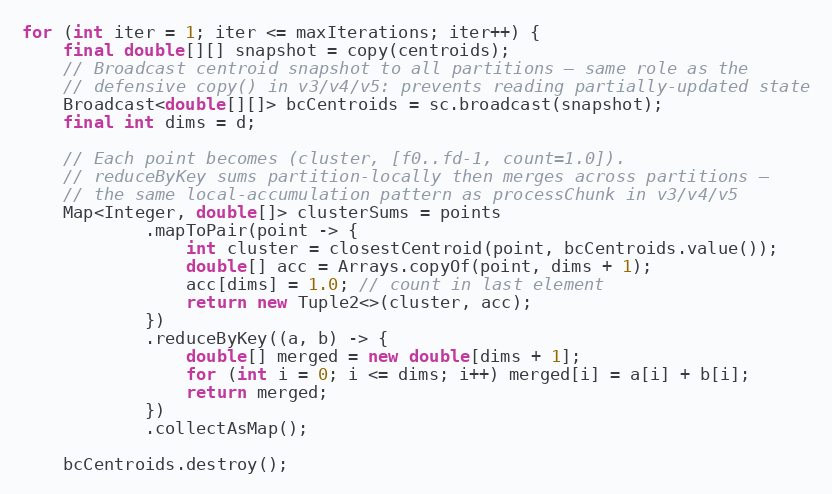
\includegraphics[width=0.85\textwidth]{img/8-spark/snippet-1}
  \caption{Broadcast do snapshot de centróides e acumulação por
           \texttt{mapToPair}+\texttt{reduceByKey} a cada iteração
           (\texttt{KMeans.cluster}, tag \texttt{v6-csv}).}
  \label{fig:snippet-spark-iteration}
\end{figure}

A Figura~\ref{fig:snippet-spark-format} mostra a única diferença de código
entre as duas variantes testadas: o formato de leitura do \texttt{DataFrame}.
Todo o restante do arquivo --- broadcast, \texttt{mapToPair}, \texttt{reduceByKey},
avaliação final --- é idêntico entre \texttt{v6-csv} e \texttt{v6-parquet}.

\begin{figure}[H]
  \centering
  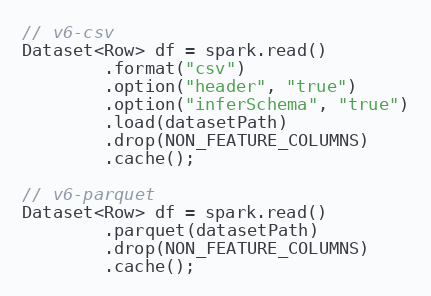
\includegraphics[width=0.7\textwidth]{img/8-spark/snippet-2}
  \caption{Única diferença de código entre \texttt{v6-csv} e
           \texttt{v6-parquet}: o formato de leitura do \texttt{DataFrame}
           (\texttt{KMeans.cluster}).}
  \label{fig:snippet-spark-format}
\end{figure}

O diagrama de classes da Figura~\ref{fig:class-diagram-spark} mostra a
estrutura da v6, bem mais simples que a das versões anteriores:
\texttt{Main} chama \texttt{KMeans.cluster}, que devolve um
\texttt{KMeansResult} (o mesmo \textit{record} usado desde a v1) e depende
diretamente de três tipos da API do Spark --- \texttt{SparkSession},
\texttt{Dataset<Row>} e \texttt{Broadcast<double[][]>}. O
\texttt{CsvDataset} das versões anteriores desaparece do grafo de
dependências: o arquivo ainda existe fisicamente no repositório da tag
\texttt{v6-csv}, mas não é mais referenciado em nenhum ponto do código.

\begin{figure}[H]
  \centering
  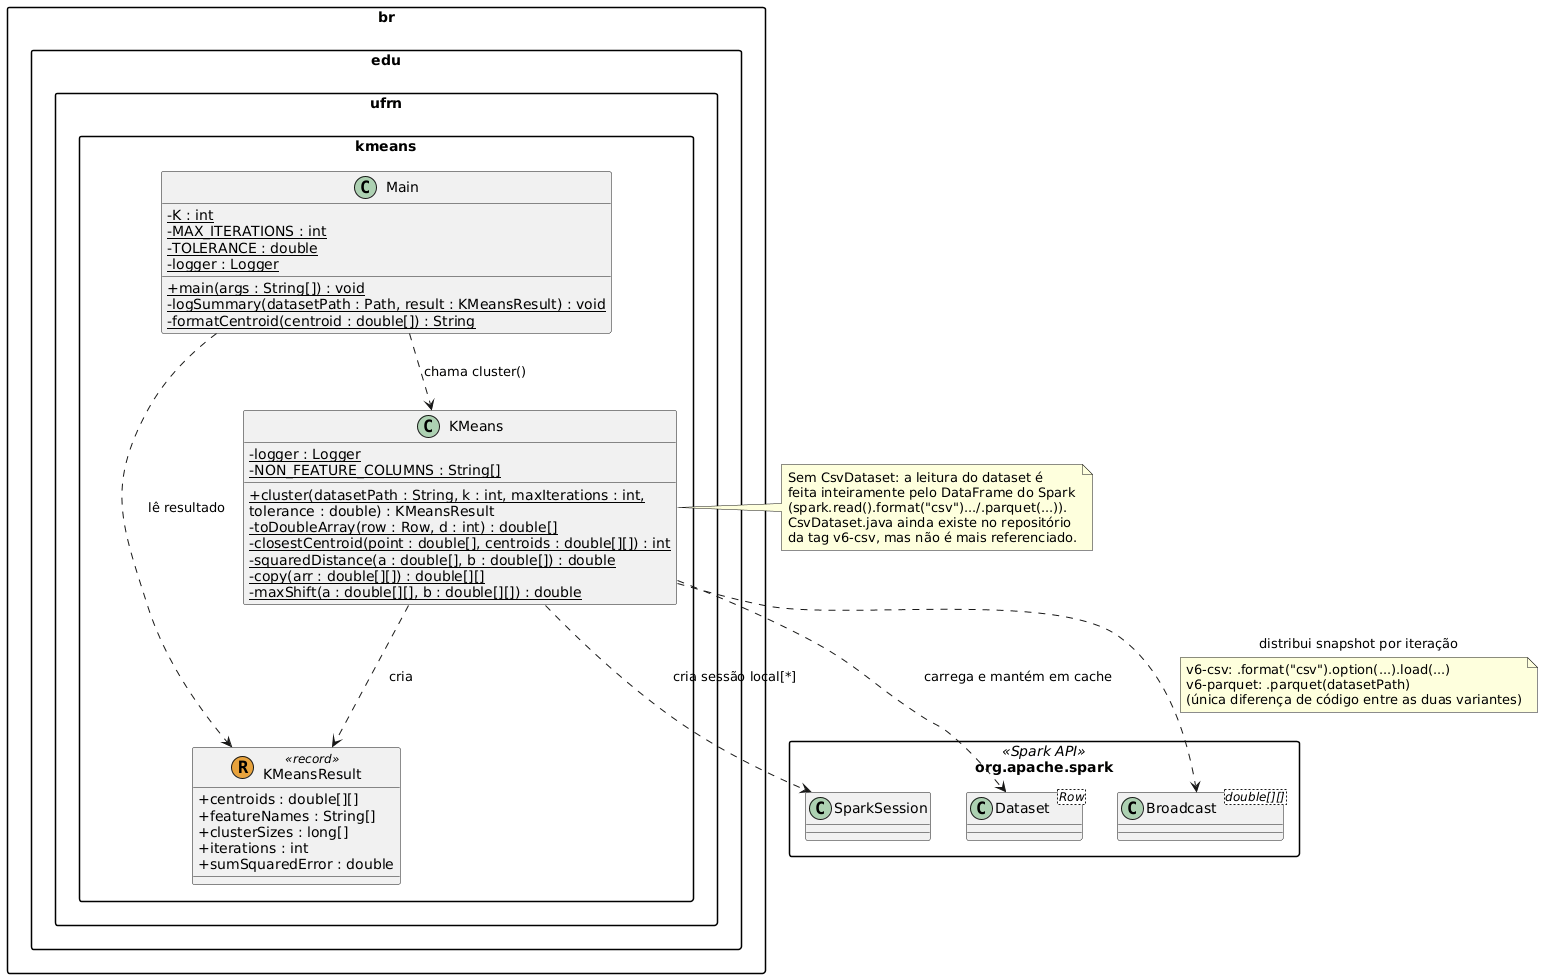
\includegraphics[width=0.95\textwidth]{img/8-spark/class-diagram}
  \caption{Diagrama de classes da v6 (Spark). \texttt{Main} e \texttt{KMeans}
           seguem estáticas como nas versões anteriores; \texttt{KMeansResult}
           é reaproveitado sem alterações. A única diferença de código entre
           \texttt{v6-csv} e \texttt{v6-parquet} está no carregamento do
           \texttt{Dataset<Row>} (ver Figura~\ref{fig:snippet-spark-format}).}
  \label{fig:class-diagram-spark}
\end{figure}

\subsubsection{Resultados}

\paragraph{Aplicabilidade das Ferramentas de Benchmark}

Nenhuma das ferramentas usadas em v1--v5 se aplica diretamente à v6.
JMH não é viável porque a inicialização de uma \texttt{SparkSession} é
pesada demais para caber no modelo de fork/iterações curtas do JMH.
JMeter não se aplica porque o Spark não foi projetado para atender
chamadas concorrentes de alta frequência --- rodar JMeter contra uma
única sessão Spark compartilhada testaria o escalonador do Spark, não o
algoritmo. JCStress não se aplica porque o modelo de execução do Spark
não tem estado mutável compartilhado entre tarefas por construção --- não
há região crítica para testar. As métricas usadas nesta versão são
\textbf{tempo de parede} (\texttt{System.nanoTime()} em torno da
execução completa) e \textbf{profile JFR}, complementado pela Spark UI
(\texttt{http://localhost:4040}) para inspeção do DAG de jobs e stages.

\paragraph{Avaliação de Tempo de Parede}

Ambas as variantes foram executadas com $k=10$ e \texttt{maxIter}=10
(sem convergência dentro desse limite), sobre o mesmo dataset de 5,75
milhões de pontos e 38 features.

\begin{table}[H]
\centering
\begin{tabular}{lrr}
\hline
\textbf{Variante} & \textbf{Tempo total (ms)} & \textbf{Tempo/iter.\textsuperscript{*} (s)} \\
\hline
v6-csv     & 34.624 & 3{,}46 \\
v6-parquet & 44.264 & 4{,}43 \\
\hline
\end{tabular}
\caption{Tempo de parede --- v6-csv vs.\ v6-parquet ($k=10$, \texttt{maxIter}=10,
mesmo dataset de 5,75 milhões de pontos; SSE final praticamente idêntico
entre as duas variantes, ver texto).
\textsuperscript{*}Estimado como tempo total $\div$ 10 iterações; não é uma
medição isolada como o B2 do JMH nas versões anteriores, apenas uma
referência aproximada de ordem de grandeza.}
\label{tab:wallclock-v6}
\end{table}

O SSE final é praticamente idêntico entre as duas variantes ---
confirmando que ambas processam o mesmo dataset e chegam ao mesmo
resultado, como esperado, já que a única diferença de código entre elas
é o formato de leitura do \texttt{DataFrame}. Contra a expectativa comum
de que um formato colunar e comprimido como o Parquet seria mais rápido
de ler que texto puro, o \textbf{Parquet ficou \textasciitilde28\% mais
lento que o CSV} nesta carga (44.264 ms contra 34.624 ms). A seção de
profile a seguir explica a causa.

\paragraph{Avaliação de Profile}

\textbf{v6-csv.} A gravação JFR totalizou 11.263 amostras de execução.

\begin{table}[H]
\centering
\small
\begin{tabular}{p{7.4cm}rrp{3cm}}
\hline
\textbf{Método} & \textbf{Amostras} & \textbf{CPU (\%)} & \textbf{Categoria} \\
\hline
\texttt{KMeans.squaredDistance}       & 1475 & 13{,}1 & Algoritmo \\
\texttt{CharInputReader.getString}    & 1179 & 10{,}5 & Parsing CSV (univocity) \\
\texttt{CompressibleColumnBuilder}    &  621 &  5{,}5 & Cache colunar (Spark) \\
\texttt{HashMap.put0}                 &  413 &  3{,}7 & Overhead Scala/Spark \\
\texttt{KMeans.closestCentroid}       &  352 &  3{,}1 & Algoritmo \\
\texttt{LineReader.readDefaultLine}   &  330 &  2{,}9 & Parsing CSV (Hadoop) \\
\hline
\end{tabular}
\caption{Hot methods na v6-csv (JFR, 11.263 amostras).}
\label{tab:jfr-hot-v6-csv}
\end{table}

Diferente da v3 --- onde nenhum evento de leitura de dataset aparece
depois da carga inicial ---, os frames de \textit{parsing} de CSV
(\texttt{AbstractCharInputReader}, \texttt{LineReader}) seguem entre os
mais amostrados mesmo depois da carga inicial. O motivo aparece na saída
de execução: o Spark registra repetidos avisos
\texttt{MemoryStore - Not enough space to cache rdd\_X in memory!} ---
sob os 4 GB de memória do driver, nem todas as partições do dataset
cabem no cache, e as partições que não couberam são \textbf{relidas e
reparseadas do CSV a cada iteração} em vez de servidas da memória. Isso
é uma diferença estrutural importante frente à v3: lá, o dataset ou cabe
inteiro no heap ou a JVM falha; aqui, o cache do Spark degrada
silenciosamente para recomputação sob pressão de memória, sem erro
explícito.

\textbf{v6-parquet.} A gravação JFR totalizou 11.016 amostras de execução.

\begin{table}[H]
\centering
\small
\begin{tabular}{p{7.4cm}rrp{3cm}}
\hline
\textbf{Método} & \textbf{Amostras} & \textbf{CPU (\%)} & \textbf{Categoria} \\
\hline
\texttt{KMeans.squaredDistance}       & 2152 & 19{,}5 & Algoritmo \\
\texttt{ParquetDictionary.decodeToLong} & 912 &  8{,}3 & Decodificação Parquet \\
\texttt{CodegenIterator.processNext}  &  813 &  7{,}4 & Codegen (Spark) \\
\texttt{CompressibleColumnBuilder}    &  757 &  6{,}9 & Cache colunar (Spark) \\
\texttt{HashMap.findNode}             &  659 &  6{,}0 & Overhead Scala/Spark \\
\texttt{KMeans.closestCentroid}       &  603 &  5{,}5 & Algoritmo \\
\texttt{ParquetDictionary.decodeToDouble} & 442 & 4{,}0 & Decodificação Parquet \\
\hline
\end{tabular}
\caption{Hot methods na v6-parquet (JFR, 11.016 amostras).}
\label{tab:jfr-hot-v6-parquet}
\end{table}

Os mesmos avisos de pressão de memória aparecem no log do v6-parquet,
mas com um comportamento diferente: em vez de descartar o bloco que não
coube, o \texttt{BlockManager} registra \texttt{"Persisting block to
disk instead"} --- o formato colunar e comprimido do Parquet muda a
forma como o Spark decide lidar com a falta de espaço no cache. Ainda
assim, o tempo total foi maior: a decodificação de dicionário/delta do
Parquet (\texttt{ParquetDictionary.decodeToLong}/\texttt{decodeToDouble})
soma uma fração relevante das amostras, um custo de CPU real que o CSV
--- apesar de mais lento para ler bruto --- não paga da mesma forma
depois que uma partição está em cache.

\textbf{Heap e GC.} O pico de heap foi de 3.891,2 MB
(\textasciitilde3,89 GB) na v6-csv e 3.993,6 MB (\textasciitilde3,99 GB)
na v6-parquet --- ambos notavelmente acima dos \textasciitilde2,6--2,76
GB de v3/v4/v5, apesar de operarem sobre o mesmo dataset bruto: as
estruturas internas do Spark (representação colunar em cache, overhead
de execução distribuída no driver e nos executores locais) somam
memória real acima dos dados em si, e ambas as variantes ficam próximas
do teto configurado de 4 GB (\texttt{-Xmx4g}) --- consistente com os
avisos de pressão de cache já discutidos. A v6-csv registrou 243
coletas de GC e a v6-parquet 124; esses números não são diretamente
comparáveis aos das versões anteriores, pois incluem sobrecarga do
próprio Spark/JVM além do algoritmo.

\subsection{Discussão}

O Spark é, neste dataset e nesta escala, \textbf{mais lento que
v3/v4/v5}: o tempo por iteração aproximado (3,46 s na v6-csv, 4,43 s na
v6-parquet) fica bem acima do B2 de v3/v4/v5 (1,60--1,98 s). O dataset
inteiro cabe confortavelmente em memória numa única máquina, e o custo
de serialização, broadcast e gerenciamento de partições distribuídas do
Spark supera qualquer benefício que o processamento distribuído
ofereceria numa escala maior. O valor pedagógico desta versão está na
mudança radical de modelo de programação --- de threads coordenadas
sobre memória compartilhada para transformações distribuídas sobre um
\texttt{Dataset} particionado --- não em um ganho de desempenho.

A comparação entre CSV e Parquet dentro da própria v6 é o achado mais
interessante desta seção: contra a intuição comum de que um formato
colunar e comprimido seria mais rápido, o \textbf{Parquet foi
\textasciitilde28\% mais lento} nesta carga, porque o custo de
decodificação de dicionário/delta por linha supera a economia de
I/O bruto. É o mesmo tipo de lição que o profile da versão serial já
havia ensinado --- \textbf{medir antes de assumir} --- agora aplicada à
escolha de formato de armazenamento em vez de à escolha de estratégia de
concorrência.

Por fim, a v6 expõe um modo de falha que nenhuma versão single-JVM tem:
sob pressão de memória, o cache do Spark degrada silenciosamente para
recomputação (relendo/reparseando partições, como visto na v6-csv) em
vez de falhar de forma explícita. Na v3, o dataset ou cabe inteiro no
heap ou a JVM lança \texttt{OutOfMemoryError} --- uma falha visível e
imediata. No Spark, a mesma restrição de memória se manifesta como uma
degradação de desempenho silenciosa, que só fica evidente ao inspecionar
o profile ou os logs de aviso do \texttt{MemoryStore}.

\newpage

\section{Discussão Final}

\subsection{Comparativo Geral das Abordagens}

O trabalho evoluiu em seis estágios principais do lado Java (serial, v2, v3, v4,
v5, v6), cada um respondendo a uma limitação do estágio anterior, além de uma
implementação paralela em Erlang usada como ponto de comparação de modelo de
concorrência.

\textbf{Serial.}
A implementação sequencial estabeleceu a baseline: uma thread lê o CSV, calcula a
distância de cada ponto aos centróides e acumula os resultados. O perfil de execução
revelou que $\approx$82\% do tempo era gasto em parsing CSV
(\texttt{FloatingDecimal.parseDouble}, \texttt{String.split}), e apenas $\approx$8\%
em computação aritmética. Isso significa que o algoritmo em si é rápido; o gargalo
é a entrada de dados.

\textbf{Concorrente v2 (platform, virtual, hybrid).}
A paralelização da fase de atribuição (lotes de 5.000 pontos, pool de $N$ workers)
não trouxe ganho de tempo por iteração: o parsing CSV seguia sequencial na thread
principal, dominando o tempo total. Os microbenchmarks mostraram B2
$\approx$60 s/op para todas as variantes, idêntico ao serial. O macrobenchmark
revelou throughput de 1,6--4,6 exec/min dependendo do número de threads JMeter
e da variante de GC.

A exploração das três variantes foi útil para entender o comportamento de cada
modelo de thread. A variante hybrid foi a mais reveladora: ao usar uma virtual thread
como coordenadora, o parsing CSV ficou invisível ao profiler --- porque a thread
suspende durante I/O em vez de consumir CPU. Isso confirmou que o gargalo não estava
na coordenação dos workers, mas na leitura do arquivo em si.

\textbf{Concorrente v3 (dados em memória).}
Carregar o dataset inteiro em \texttt{double[][]} antes do loop de iterações
eliminou o parsing CSV das medições. B2 caiu de $\approx$60 s para $\approx$1{,}6 s
($\approx$37$\times$); o throughput saltou de $\approx$1,6 para $\approx$52
exec/min com 1 thread JMeter. O perfil não registrou nenhum evento de leitura de
arquivo durante o clustering. O custo foi o aumento do heap de $\approx$250 MB
para $\approx$2{,}7 GB.

\textbf{Concorrente v4 (concorrência estruturada).}
A v4 substitui o par \texttt{ExecutorService} + \texttt{CountDownLatch} da v3
por \texttt{StructuredTaskScope} e \texttt{ScopedValue} (JEP 480/446), corrigindo uma
lacuna estrutural real: exceções lançadas dentro de uma tarefa de worker, antes
sem canal de propagação de volta à coordenadora, passam a propagar corretamente
via \texttt{scope.join()}, que também cancela subtarefas irmãs automaticamente.
O preço é um aumento modesto no custo por iteração (B2: 1{,}60 s $\to$ 1{,}98 s,
$\approx$24\%) e no throughput (52,5--62,3 $\to$ 45,8--52,0 exec/min), atribuído
à imaturidade de compilação das APIs de \textit{preview}. O confinamento local
por tarefa permanece inalterado e validado por JCStress.

\textbf{Concorrente v5 (fork/join).}
A v5 troca o particionamento fixo em $N$ chunks por divisão-e-conquista
recursiva com \texttt{RecursiveTask} e \textit{work-stealing}. Os números ficam
muito próximos aos da v4 (B2 = 1{,}78 s; throughput 46,4--52,4 exec/min) --- o
dataset uniforme deste trabalho não oferece o desbalanceamento entre partições
que o \textit{work-stealing} precisaria para mostrar vantagem real. O achado
mais relevante é a variância elevada de B1 ($\pm$16{,}08 s), ecoando o mesmo
efeito já visto na v2-virtual: pools de tarefas pensados para trabalho que
cede o processador introduzem ruído de escalonamento em cargas puramente
aritméticas que nunca bloqueiam.

\textbf{Spark (v6, processamento distribuído).}
A v6 abandona o modelo de memória compartilhada em favor de um
\texttt{Dataset<Row>} particionado gerenciado pelo Spark, com
\texttt{mapToPair}+\texttt{reduceByKey} por iteração e broadcast do snapshot de
centróides. Nem JMH, nem JMeter, nem JCStress se aplicam a este modelo; a
métrica usada foi tempo de parede. O tempo por iteração aproximado
($\approx$3{,}46 s no CSV; $\approx$4{,}43 s no Parquet) fica acima do B2 de
v3--v5 --- o custo de coordenação distribuída supera o benefício em um dataset
que cabe confortavelmente em uma única máquina. O achado mais interessante foi
contraintuitivo: o Parquet, formato colunar e comprimido, foi
$\approx$28\% \textit{mais lento} que o CSV bruto nesta carga, pela sobrecarga
de decodificação de dicionário/delta por linha. O cache do Spark também expôs
um modo de falha ausente nas versões single-JVM: sob pressão de memória,
partições não cacheadas são silenciosamente relidas/reparseadas em vez de
causar um erro explícito.

\textbf{Erlang concorrente (modelo de atores, dados em memória).}
Esta implementação parte do mesmo ponto que a v3 (dados em memória) e não foi
estendida para acompanhar v4--v6, que são extensões específicas do lado Java;
a comparação a seguir é sempre contra a v3. Distribui chunks entre 16 workers
BEAM, sem memória compartilhada. O custo por
iteração ficou em $\approx$21{,}3 s ($\approx$66$\times$ acima do Java v3 --- ver Tabela~\ref{tab:bench-erlang-vs-v3}). O gargalo é
a aritmética por ponto: B3 e B4 são 113--165$\times$ mais lentos que em Java,
pois a BEAM desempacota floats de binários sem vetorização SIMD. Os schedulers
operaram a 45{,}7\% de utilização — a redução centralizada serializa parte de
cada iteração.

A Tabela~\ref{tab:comparativo-geral} resume os principais números de cada abordagem.

\begin{table}[H]
\centering
\small
\begin{tabular}{lrrrr}
\hline
\textbf{Abordagem} & \textbf{B2 (s/op)} & \textbf{Throughput 1t} & \textbf{Throughput 16t} & \textbf{Heap pico} \\
\hline
Serial             & 60{,}05 & 1{,}56/min\textsuperscript{*} & 4{,}66/min\textsuperscript{*} & $\approx$250 MB \\
v2-platform        & 60{,}69 & 1{,}65/min & 4{,}49/min & $\approx$250 MB \\
v2-virtual         & 71{,}61 & 1{,}62/min & 4{,}55/min & $\approx$250 MB \\
v2-hybrid          & 60{,}44 & 1{,}60/min & 4{,}53/min & $\approx$250 MB \\
v3                 &  1{,}60 & 52{,}5/min & 62{,}3/min & $\approx$2{,}7 GB \\
v4                 &  1{,}98 & 45{,}8/min & 52{,}0/min & $\approx$2{,}76 GB \\
v5                 &  1{,}78 & 46{,}4/min & 52{,}4/min & $\approx$2{,}56 GB \\
v6-csv             & 3{,}46\textsuperscript{\ddag} & N/A\textsuperscript{\ddag} & N/A\textsuperscript{\ddag} & $\approx$3{,}89 GB \\
v6-parquet         & 4{,}43\textsuperscript{\ddag} & N/A\textsuperscript{\ddag} & N/A\textsuperscript{\ddag} & $\approx$3{,}99 GB \\
Erlang (16 workers)& 21{,}27\textsuperscript{\dag} &     N/A    &     N/A    & $\approx$1{,}75 GB \\
\hline
\end{tabular}
\caption{Comparativo geral entre abordagens (B2 = custo por iteração; throughput = exec/min, JMeter G1GC exceto v3--v5 com ParallelGC; Erlang sem macrobenchmark HTTP; v6 sem JMH/JMeter, ver texto).
\textsuperscript{*}Serial: $N$ instâncias independentes executadas em paralelo pelo JMeter (sem concorrência interna); ver Tabela~\ref{tab:jmeter-serial-java}.
\textsuperscript{\dag}Erlang B2 estimado como B1\,/\,\texttt{maxIter} (106.344{,}7\,ms\,÷\,5\,÷\,1000); sem benchmark B2 dedicado.
\textsuperscript{\ddag}v6: sem JMH dedicado; B2 estimado como tempo de parede total $\div$ 10 iterações
(ver Tabela~\ref{tab:wallclock-v6} na Seção~\ref{sec:spark}); sem macrobenchmark JMeter --- Spark
não foi projetado para atender chamadas concorrentes de alta frequência.}
\label{tab:comparativo-geral}
\end{table}

\begin{figure}[H]
    \centering
    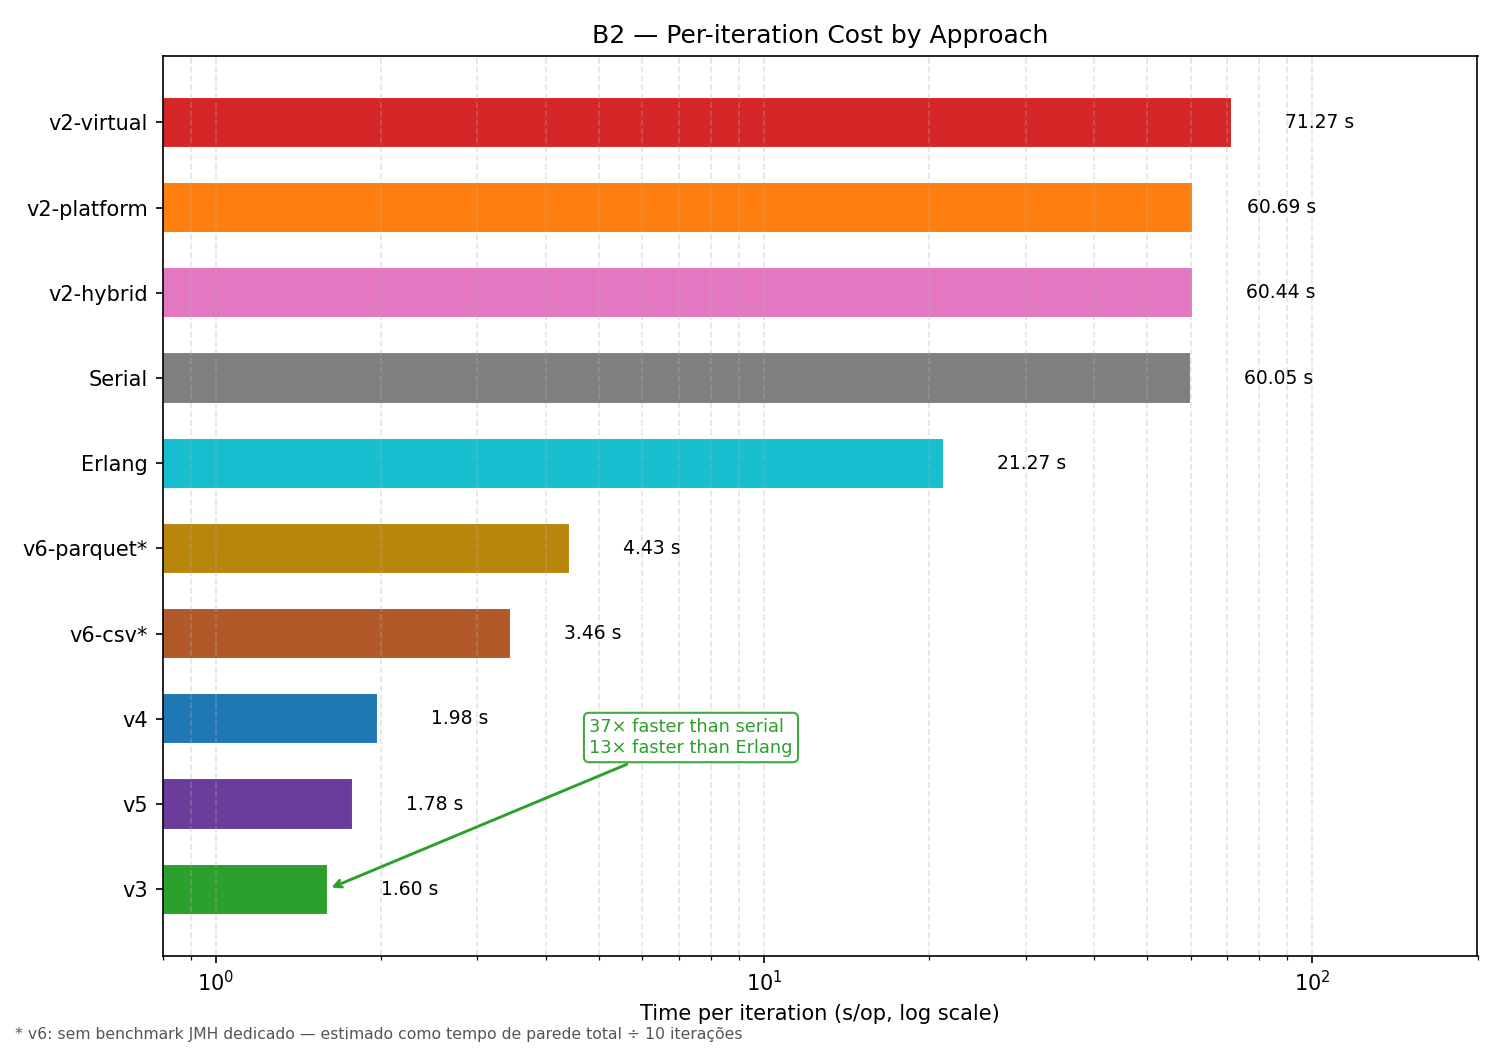
\includegraphics[width=0.85\textwidth]{img/charts/chart1_b2_cost}
    \caption{Custo por iteração (B2) em escala logarítmica, todas as abordagens.
             As variantes v2 e Serial ficam acima de 60 s/op, dominadas pelo
             parsing CSV. Erlang fica em 21{,}27 s/op ($\approx$13$\times$
             acima da v3) pelo custo aritmético da BEAM sem vetorização SIMD.
             v6-csv e v6-parquet (marcadas com {*}) não têm B2 dedicado ---
             o valor mostrado é o tempo de parede total dividido por 10
             iterações (ver Tabela~\ref{tab:wallclock-v6} na
             Seção~\ref{sec:spark}) --- e ainda assim ficam acima de v3, v4 e
             v5, que caem para a faixa de 1{,}6--2,0 s/op ao eliminar a
             coordenação distribuída. v3 segue sendo a mais rápida, $37\times$
             mais rápida que o Serial.}
    \label{fig:chart-b2-cost}
\end{figure}

O \texttt{chart2\_macro\_throughput.png} (Seção~\ref{sec:concurrent-x}) cobre
apenas Serial, v2 e v3 e foi mantido como está. A Figura~\ref{fig:chart-throughput-v3-v5}
é um gráfico novo e independente, comparando diretamente v3, v4 e v5 --- as
três únicas versões com macrobenchmark no mesmo coletor (ParallelGC), o que
torna a comparação direta sem ressalvas de GC.

\begin{figure}[H]
    \centering
    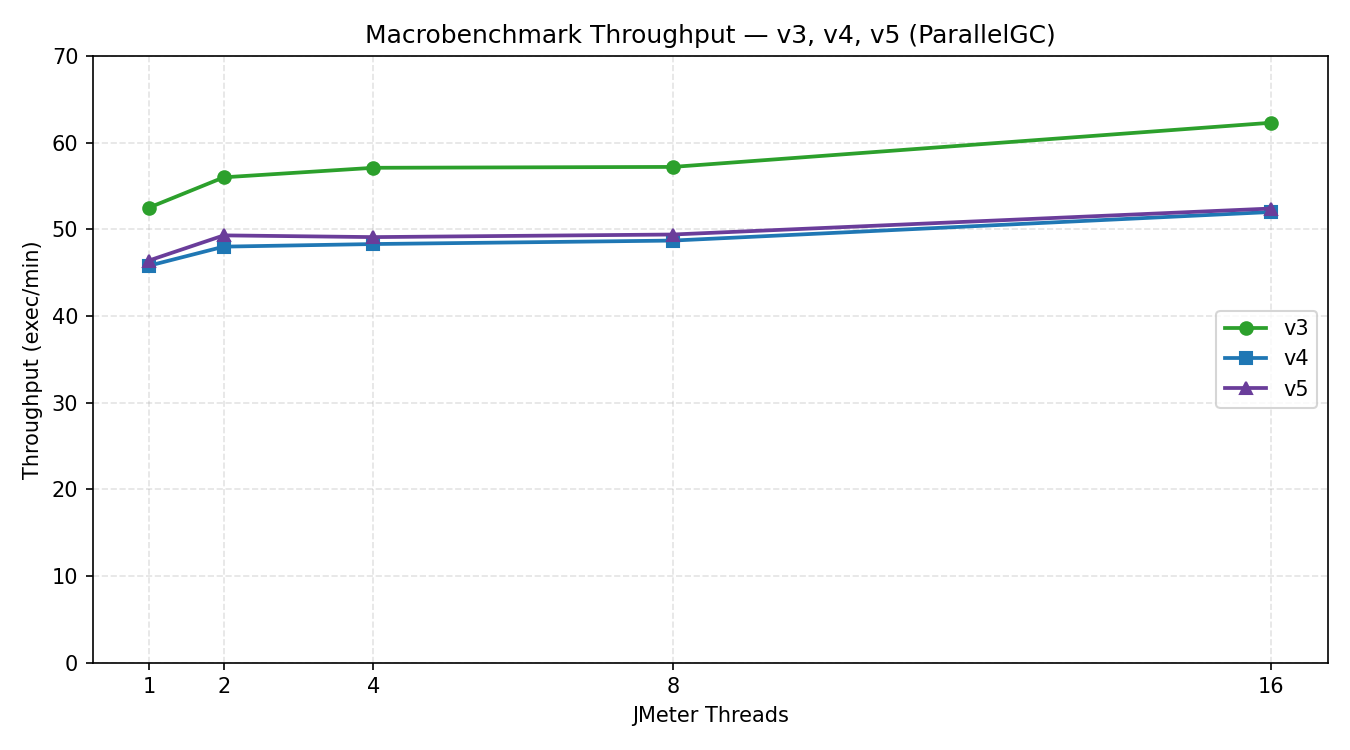
\includegraphics[width=0.85\textwidth]{img/charts/chart5_throughput_v3_v5}
    \caption{Throughput (execuções/min) por número de threads JMeter --- v3,
             v4 e v5, todas com ParallelGC. v4 e v5 ficam muito próximas entre
             si e abaixo da v3 em todos os níveis de carga, consistente com o
             aumento de custo por iteração (B2) discutido nas
             Seções~\ref{sec:structured} e~\ref{sec:forkjoin}. v6 não aparece
             neste gráfico --- não há macrobenchmark JMeter para o Spark (ver
             Seção~\ref{sec:spark}).}
    \label{fig:chart-throughput-v3-v5}
\end{figure}

\subsection{Pontos Positivos e Negativos de Cada Abordagem}

\subsubsection*{Serial}

\textbf{Positivos.}
Simples de implementar e depurar. Ausência de condições de corrida por definição.
Baixo consumo de memória. Serve como baseline clara para medir ganhos das versões
concorrentes.

\textbf{Negativos.}
Subutiliza processadores multi-core. A thread principal acumula os dois papéis
(I/O e computação) sem possibilidade de sobreposição.

\subsubsection*{v2 --- Concorrência com Lotes e Futures}

\textbf{Positivos.}
Paraleliza a fase computacionalmente intensiva (atribuição de pontos a centróides)
sem exigir sincronização explícita, graças à acumulação local por worker. A
estrutura de \texttt{Future.get()} fornece garantia de happens-before clara. A
variante hybrid demonstrou que virtual threads são adequadas para coordenadores
que alternam entre I/O e espera.

\textbf{Negativos.}
O parsing CSV sequencial na thread principal continua sendo o gargalo, tornando o
ganho da paralelização invisível no tempo de parede. A criação de objetos
\texttt{List.copyOf} e \texttt{PartialResult} por lote gera pressão de GC.
A virtual thread em tarefas CPU-bound de curta duração introduz variância elevada
no JMH (até $\pm$260 s), pois o \texttt{ForkJoinPool} não foi projetado para
tarefas que nunca bloqueiam.

\subsubsection*{Erlang --- Concorrência por Atores}

\textbf{Positivos.}
Race conditions são impossíveis por construção: processos não compartilham memória,
eliminando a necessidade de locks, atomics ou \texttt{volatile}. O GC é por
processo e sem pausas globais: nenhum stop-the-world afeta todos os workers
simultaneamente. Workers de longa duração mantêm os chunks em seus heaps locais
sem overhead de cópia, graças à semântica de referência dos binários grandes da
BEAM. O modelo de atores escala naturalmente para clusters distribuídos sem
mudança de paradigma.

\textbf{Negativos.}
A aritmética por ponto é 113--165$\times$ mais lenta que em Java: a BEAM
desempacota floats de binários elemento a elemento sem geração de código SIMD.
Os schedulers operaram a 45{,}7\% de utilização: a redução centralizada no processo
principal (\texttt{collect\_partial} + recompute) é um gargalo serial que mantém
os workers ociosos $\approx$54\% do tempo. A reconstrução de listas de somas via
\texttt{update\_nth} gerou 2{,}1 milhões de coletas GC por alocação excessiva de
células de lista --- custo inexistente em Java, que acumula em arrays mutáveis
locais. A ausência de servidor HTTP inviabilizou a comparação de throughput com
JMeter nas mesmas condições das versões Java.

\subsubsection*{v3 --- Dados em Memória com CountDownLatch}

\textbf{Positivos.}
Elimina o I/O das iterações, revelando o verdadeiro custo computacional do algoritmo.
A divisão em $N$ chunks fixos é mais simples que a criação dinâmica de lotes:
sem \texttt{List.copyOf}, sem \texttt{Future} por lote. \texttt{CountDownLatch}
é mais direto que coletar e iterar sobre uma lista de \texttt{Future}s. O
\texttt{KMeansSampler} com \texttt{sharedPoints} estático permite que múltiplos
threads JMeter compartilhem os dados sem alocar múltiplos GBs por thread.

\textbf{Negativos.}
O dataset inteiro precisa caber na heap ($\approx$1{,}75 GB para $\approx$5{,}75
milhões de pontos com 38 features). Isso inviabiliza a abordagem para datasets
maiores sem particionamento externo. O tempo de inicialização (leitura única do
CSV) não é contabilizado nas métricas, o que pode ser enganoso se o processo for
reiniciado frequentemente.

\subsubsection*{v4 --- Concorrência Estruturada}

\textbf{Positivos.}
Corrige uma lacuna estrutural real da v3: exceções de worker agora propagam
corretamente via \texttt{scope.join()}, com cancelamento automático de
subtarefas irmãs. \texttt{ScopedValue} substitui a passagem de centróides por
parâmetro com uma alternativa mais segura que \texttt{ThreadLocal} para virtual
threads filhas. O confinamento local por tarefa é preservado sem alterações e
segue validado por JCStress.

\textbf{Negativos.}
Custo mensurável em relação à v3: B2 sobe $\approx$24\% (1{,}60 s $\to$
1{,}98 s) e o throughput cai em todos os níveis de carga testados. As APIs de
\textit{preview} exigem \texttt{--enable-preview} em toda a cadeia de build e
execução (compilação, JMH, JCStress, JMeter).

\subsubsection*{v5 --- Fork/Join}

\textbf{Positivos.}
Introduz \textit{work-stealing} a nível de tarefa: divisão recursiva por
limiar permite que threads ociosas roubem subtarefas de outras, vantagem
estrutural em cargas desbalanceadas entre partições. B2 melhora levemente
frente à v4 (1{,}78 s).

\textbf{Negativos.}
Sem ganho aparente neste dataset uniforme --- números de throughput quase
idênticos aos da v4. A variância de B1 ($\pm$16{,}08 s) é a maior desde a
v2-virtual, mesmo efeito de ruído de agendamento em tarefas CPU-bound sobre
\texttt{ForkJoinPool}. Nenhum teste de sensibilidade ao limiar de divisão foi
realizado.

\subsubsection*{v6 --- Spark (Processamento Distribuído)}

\textbf{Positivos.}
Modelo de programação radicalmente diferente das versões anteriores
(transformações distribuídas sobre um \texttt{Dataset} particionado em vez de
threads coordenadas sobre memória compartilhada), relevante para cargas que
não cabem em uma única máquina. \texttt{mapToPair}+\texttt{reduceByKey}
expressa o mesmo padrão de acumulação local das versões anteriores em um
paradigma declarativo.

\textbf{Negativos.}
Mais lento que v3--v5 neste dataset, que cabe confortavelmente em memória numa
única máquina --- o overhead de coordenação distribuída não se paga nesta
escala. JMH, JMeter e JCStress não se aplicam, reduzindo a comparabilidade
direta com as versões anteriores. Sob pressão de memória, o cache degrada
silenciosamente para recomputação em vez de falhar de forma explícita (ao
contrário da v3, que ou cabe no heap ou lança \texttt{OutOfMemoryError}).
Contraintuitivamente, o formato Parquet foi $\approx$28\% mais lento que o CSV
nesta carga.

\subsection{Lições Aprendidas}

\textbf{Medir antes de paralelizar.}
O JFR mostrou que $\approx$82\% do tempo serial era parsing CSV. Paralelizar apenas o
loop aritmético ($\approx$8\% do total) dificilmente produziria ganho perceptível sem
antes eliminar o gargalo de I/O.

\textbf{Gargalos migram.}
Com o I/O eliminado na v3, o gargalo passou a ser \texttt{squaredDistance} e
\texttt{closestCentroid}. Em iterações futuras, esse é o ponto a otimizar
(SIMD, vetorização, redução de dimensionalidade).

\textbf{Virtual threads não são bala de prata para CPU-bound.}
Virtual threads brilham com bloqueio I/O, liberando o carrier para reuso.
Em tarefas puramente aritméticas, não oferecem vantagem sobre platform threads
e podem introduzir variância de escalonamento indesejada.

\textbf{Acumulação local elimina sincronização.}
O padrão map-reduce local — cada worker acumula em arrays próprios, a thread
coordenadora reduz no final — evitou locks, atomics e \texttt{volatile}.
O JCStress confirmou a ausência de race conditions nas operações reais e sua
presença ao remover a proteção (JCS3, JCS4).

\textbf{O modelo de atores não é universal.}
K-Means é CPU-bound com comunicação mínima entre iterações — perfil que favorece
memória compartilhada. O modelo de atores Erlang brilha em sistemas distribuídos,
I/O intensivo e alta disponibilidade, onde o isolamento de processos é vantagem
estrutural, não custo.

\textbf{Robustez estrutural tem custo mensurável.}
A v4 trocou uma lacuna real de tratamento de erro (exceção de worker
silenciosamente mascarada na v3) por um aumento de $\approx$24\% no custo por
iteração --- APIs mais seguras (\texttt{StructuredTaskScope},
\texttt{ScopedValue}) não são gratuitas enquanto ainda são \textit{preview}.

\textbf{\textit{Work-stealing} não ajuda cargas uniformes.}
A v5 não superou a v4 neste dataset sintético e bem distribuído entre
partições --- \textit{work-stealing} só compensa seu overhead de agendamento
quando há desbalanceamento real de carga, o que não é o caso aqui.

\textbf{Mudar o modelo de execução muda o cálculo de custo-benefício.}
O Spark (v6) foi mais lento que todas as versões Java de memória compartilhada
nesta escala --- o overhead de coordenação distribuída (serialização,
broadcast, gerenciamento de partições) só se paga quando o dataset não cabe
em uma única máquina.

\textbf{Formato de armazenamento também é uma variável de desempenho.}
Contra a intuição de que Parquet (colunar, comprimido) seria mais rápido que
CSV, ele foi $\approx$28\% mais lento nesta carga --- o custo de decodificação
de dicionário/delta por linha superou a economia de I/O bruto. Mais uma
confirmação da lição "medir antes de assumir".

\textbf{Sistemas distribuídos falham de formas que sistemas single-JVM não falham.}
Sob pressão de memória, o cache do Spark degrada silenciosamente para
recomputação em vez de lançar um erro explícito --- ao contrário da v3, onde o
dataset ou cabe no heap ou a JVM falha de forma visível.

\newpage

\section{Repositórios}

Os repositórios do projeto estão disponíveis no GitHub. Cada um corresponde a um
componente do trabalho e possui tags marcando as versões entregues.

\subsection*{Implementação Java}

Contém o algoritmo K-Means serial e as variantes concorrentes (v2-platform,
v2-virtual, v2-hybrid, v3), além dos benchmarks JMH, testes JCStress, macrobenchmark
JMeter e profile JFR.

\begin{itemize}
    \item \textbf{URL:} \url{https://github.com/rarycoringa/concurrent-kmeans-java-application}
    \item \textbf{Tags:} \texttt{v1} (serial), \texttt{v2-platform}, \texttt{v2-virtual},
          \texttt{v2-hybrid}, \texttt{v3} (dados em memória)
\end{itemize}

\subsection*{Implementação Erlang}

Contém a implementação concorrente em Erlang com o modelo de atores da BEAM,
benchmarks com \texttt{timer:tc} e profile com \texttt{erlang:statistics}.

\begin{itemize}
    \item \textbf{URL:} \url{https://github.com/rarycoringa/concurrent-kmeans-erlang-application}
    \item \textbf{Tags:} \texttt{v1} (concorrente, dados em memória)
\end{itemize}

\subsection*{Gerador de Dataset}

Scripts Python para geração do dataset sintético de pedidos utilizado em todos os
experimentos ($\approx$5{,}75 milhões de linhas, 38 features).

\begin{itemize}
    \item \textbf{URL:} \url{https://github.com/rarycoringa/concurrent-kmeans-dataset-generator-python-scripts}
    \item \textbf{Tags:} nenhuma
\end{itemize}


\end{document}
